\documentclass[compress]{beamer}
\usepackage{ifthen,verbatim}

\newcommand{\isnote}{}
\xdefinecolor{lightyellow}{rgb}{1.,1.,0.25}
\xdefinecolor{darkblue}{rgb}{0.1,0.1,0.7}

%% Uncomment this to get annotations
%% \def\notes{\addtocounter{page}{-1}
%%            \renewcommand{\isnote}{*}
%% 	   \beamertemplateshadingbackground{lightyellow}{white}
%%            \begin{frame}
%%            \frametitle{Notes for the previous page (page \insertpagenumber)}
%%            \itemize}
%% \def\endnotes{\enditemize
%% 	      \end{frame}
%%               \beamertemplateshadingbackground{white}{white}
%%               \renewcommand{\isnote}{}}

%% Uncomment this to not get annotations
\def\notes{\comment}
\def\endnotes{\endcomment}

\setbeamertemplate{navigation symbols}{}
\setbeamertemplate{headline}{\mbox{ } \hfill
\begin{minipage}{5.5 cm}
\vspace{-0.75 cm} \small
\end{minipage} \hfill
\begin{minipage}{4.5 cm}
\vspace{-0.75 cm} \small
\begin{flushright}
\ifthenelse{\equal{\insertpagenumber}{1}}{}{Jim Pivarski \hspace{0.2 cm} \insertpagenumber\isnote/\pageref{numpages}}
\end{flushright}
\end{minipage}\mbox{\hspace{0.2 cm}}\includegraphics[height=1 cm]{../cmslogo} \hspace{0.1 cm} \includegraphics[height=1 cm]{../tamulogo} \hspace{0.01 cm} \vspace{-1.05 cm}}

\begin{document}
\begin{frame}
\vfill
\begin{center}
\textcolor{darkblue}{\Large A first look at CRAFT-2009 alignment tracks}

\vfill
\begin{columns}
\column{0.3\linewidth}
\begin{center}
\large
\textcolor{darkblue}{Jim Pivarski}
\end{center}
\end{columns}

\begin{columns}
\column{0.3\linewidth}
\begin{center}
\scriptsize
{\it Texas A\&M University}
\end{center}
\end{columns}

\vfill
 1 September, 2009

\end{center}
\end{frame}

%% \begin{notes}
%% \item This is the annotated version of my talk.
%% \item If you want the version that I am presenting, download the one
%% labeled ``slides'' on Indico (or just ignore these yellow pages).
%% \item The annotated version is provided for extra detail and a written
%% record of comments that I intend to make orally.
%% \item Yellow notes refer to the content on the {\it previous} page.
%% \item All other slides are identical for the two versions.
%% \end{notes}

\small

\begin{frame}
\frametitle{What's new?}
\begin{itemize}\setlength{\itemsep}{0.25 cm}
\item Alignment framework automated \hfill (V.~Khotilovich, TAMU)
\begin{itemize}
\item choice of what should be flexible and what should be fixed based on CRAFT-08 analysis
\end{itemize}
\item First alignments of CRAFT-09 performed
\begin{itemize}\setlength{\itemsep}{0.1 cm}
\item observed few-mm translations, rotations in barrel wheels
\item and more interesting features in endcaps (subject of this talk)
\end{itemize}
\item Interesting features in endcaps
\begin{itemize}\setlength{\itemsep}{0.1 cm}
\item unlike CRAFT-08 (or 2\_2\_11 CSCSkim reconstruction), we find
  globalMuons on both the bottoms {\it and tops} of the stations
\item even for top$+$bottom trigger
\item $\phi_y$ angles of individual chambers reproduced from 2008
  $\to$ 2009, but with more complete coverage in 2009
\item alternating even-odd structure in $r\phi$ residuals???
\item ME$+$4/2 are well-aligned (with very low statistics :)
\end{itemize}
\end{itemize}
%% \hspace{-0.83 cm} \textcolor{darkblue}{\Large Outline2}
\end{frame}

\begin{frame}
\frametitle{Reminder of method}

\begin{itemize}
\item Propagate tracks from the tracker into the endcap
\item Compare position and angle of track intersection with segment

{\scriptsize (actually linear-fit of single-hit residuals, to account for possible curvature)}

\item ``$r\phi$'' = direction perpendicular to CSC strips (no granularity)

\item $\Delta r\phi$, $\Delta \frac{d(r\phi)}{dz}$ residuals interpreted as $r\phi$ translation, $\phi_y$ rotation
\end{itemize}

\begin{columns}
\column{0.6\linewidth}
\begin{center}
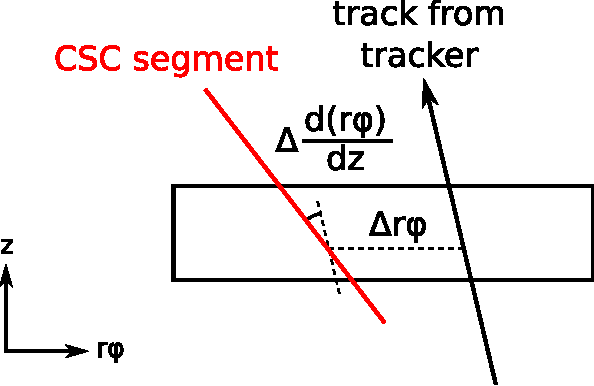
\includegraphics[width=0.7\linewidth]{explanation.pdf}
\end{center}

\column{0.4\linewidth}
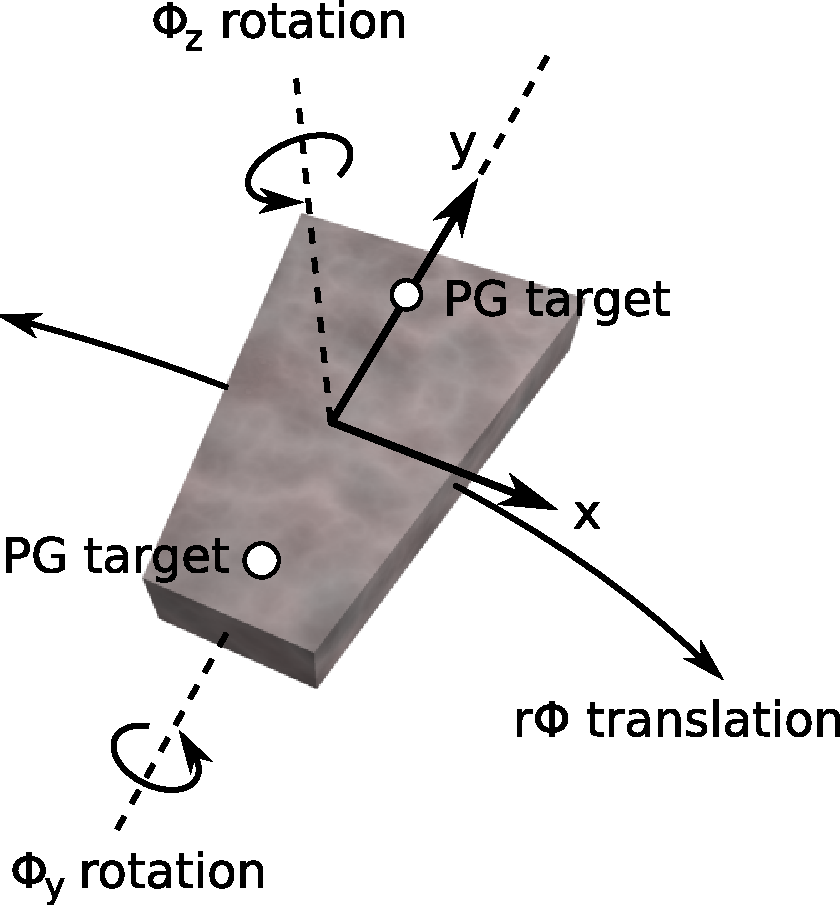
\includegraphics[width=\linewidth]{csc_coordinates.pdf}
\end{columns}
\end{frame}

\begin{frame}
\frametitle{New data are more complete}
\framesubtitle{Chamber angles are independent of disk misalignment, more reproducible}

\vspace{0.2 cm}
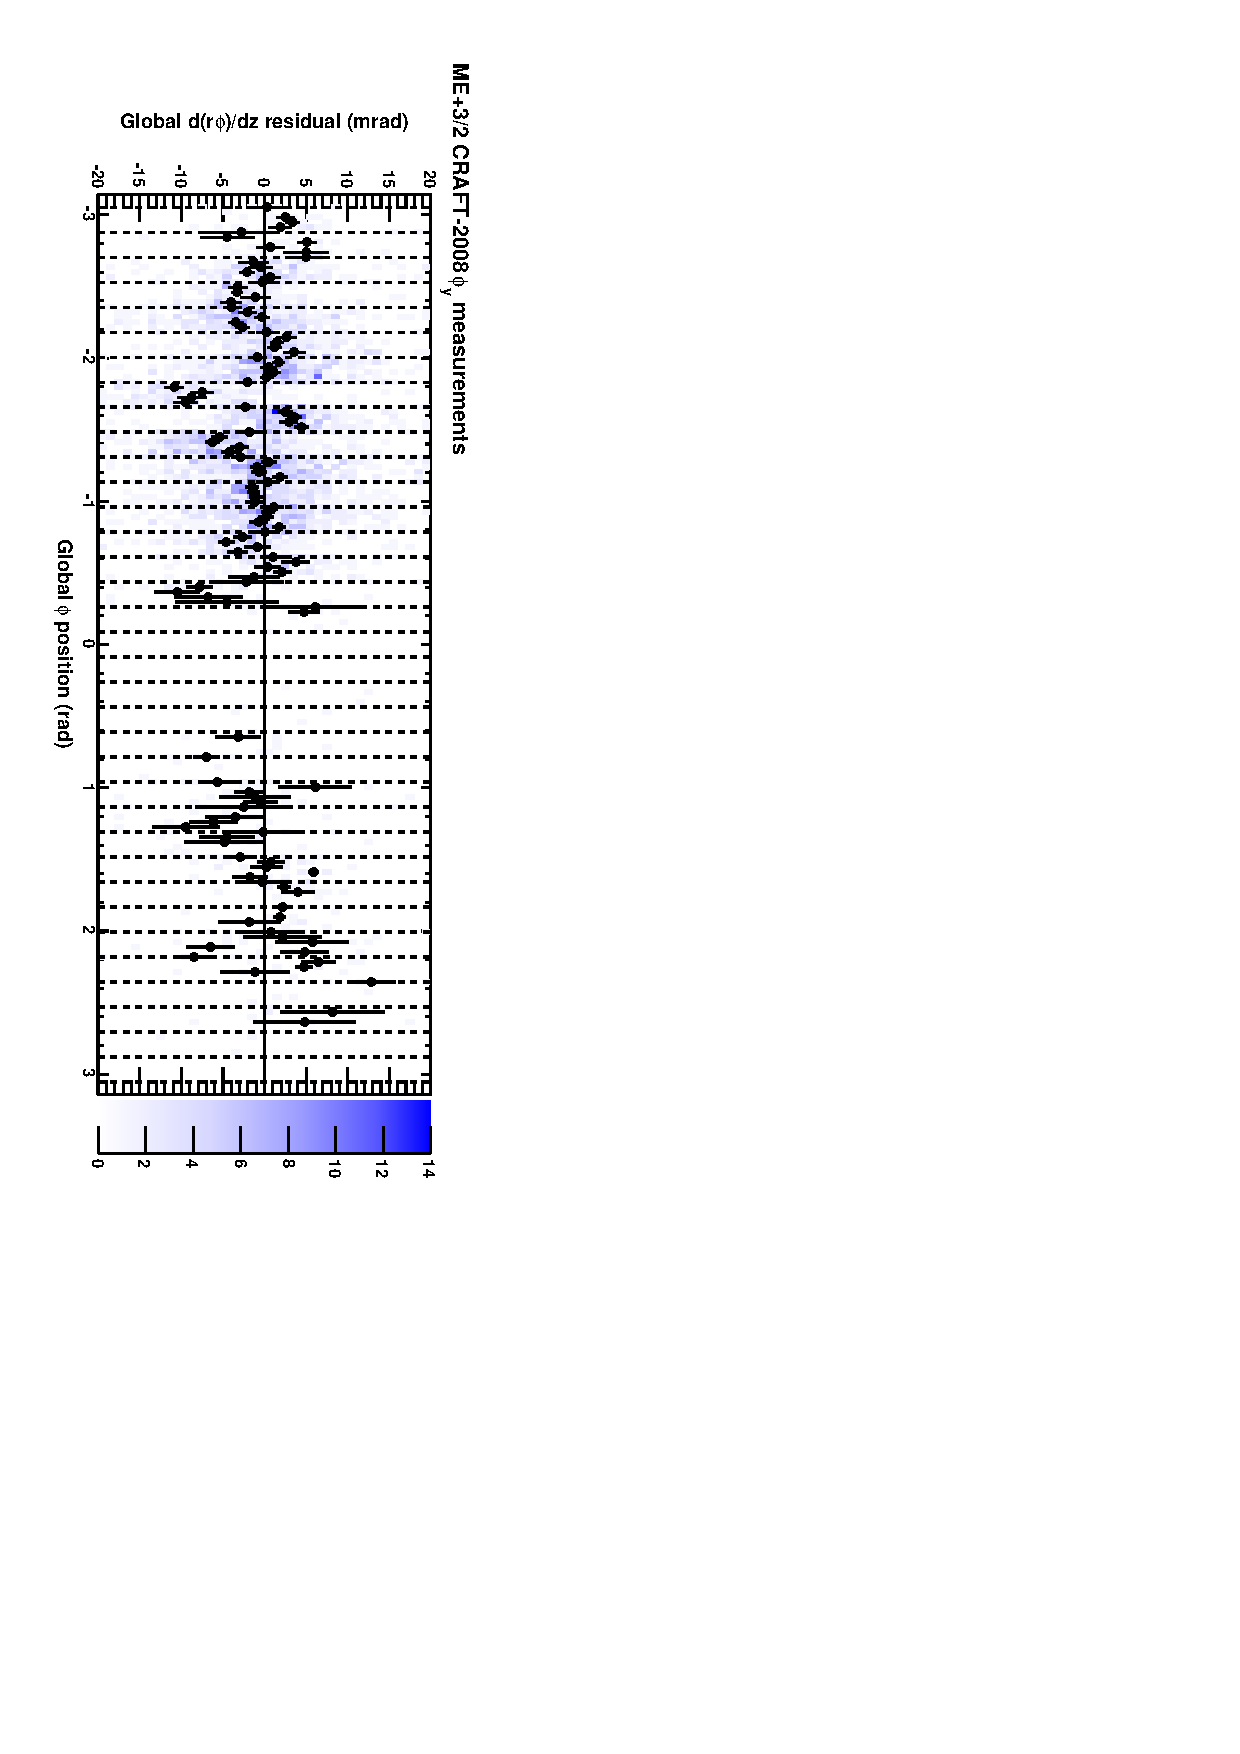
\includegraphics[height=\linewidth, angle=90]{correspondance_2008_mep32_phiy.pdf}

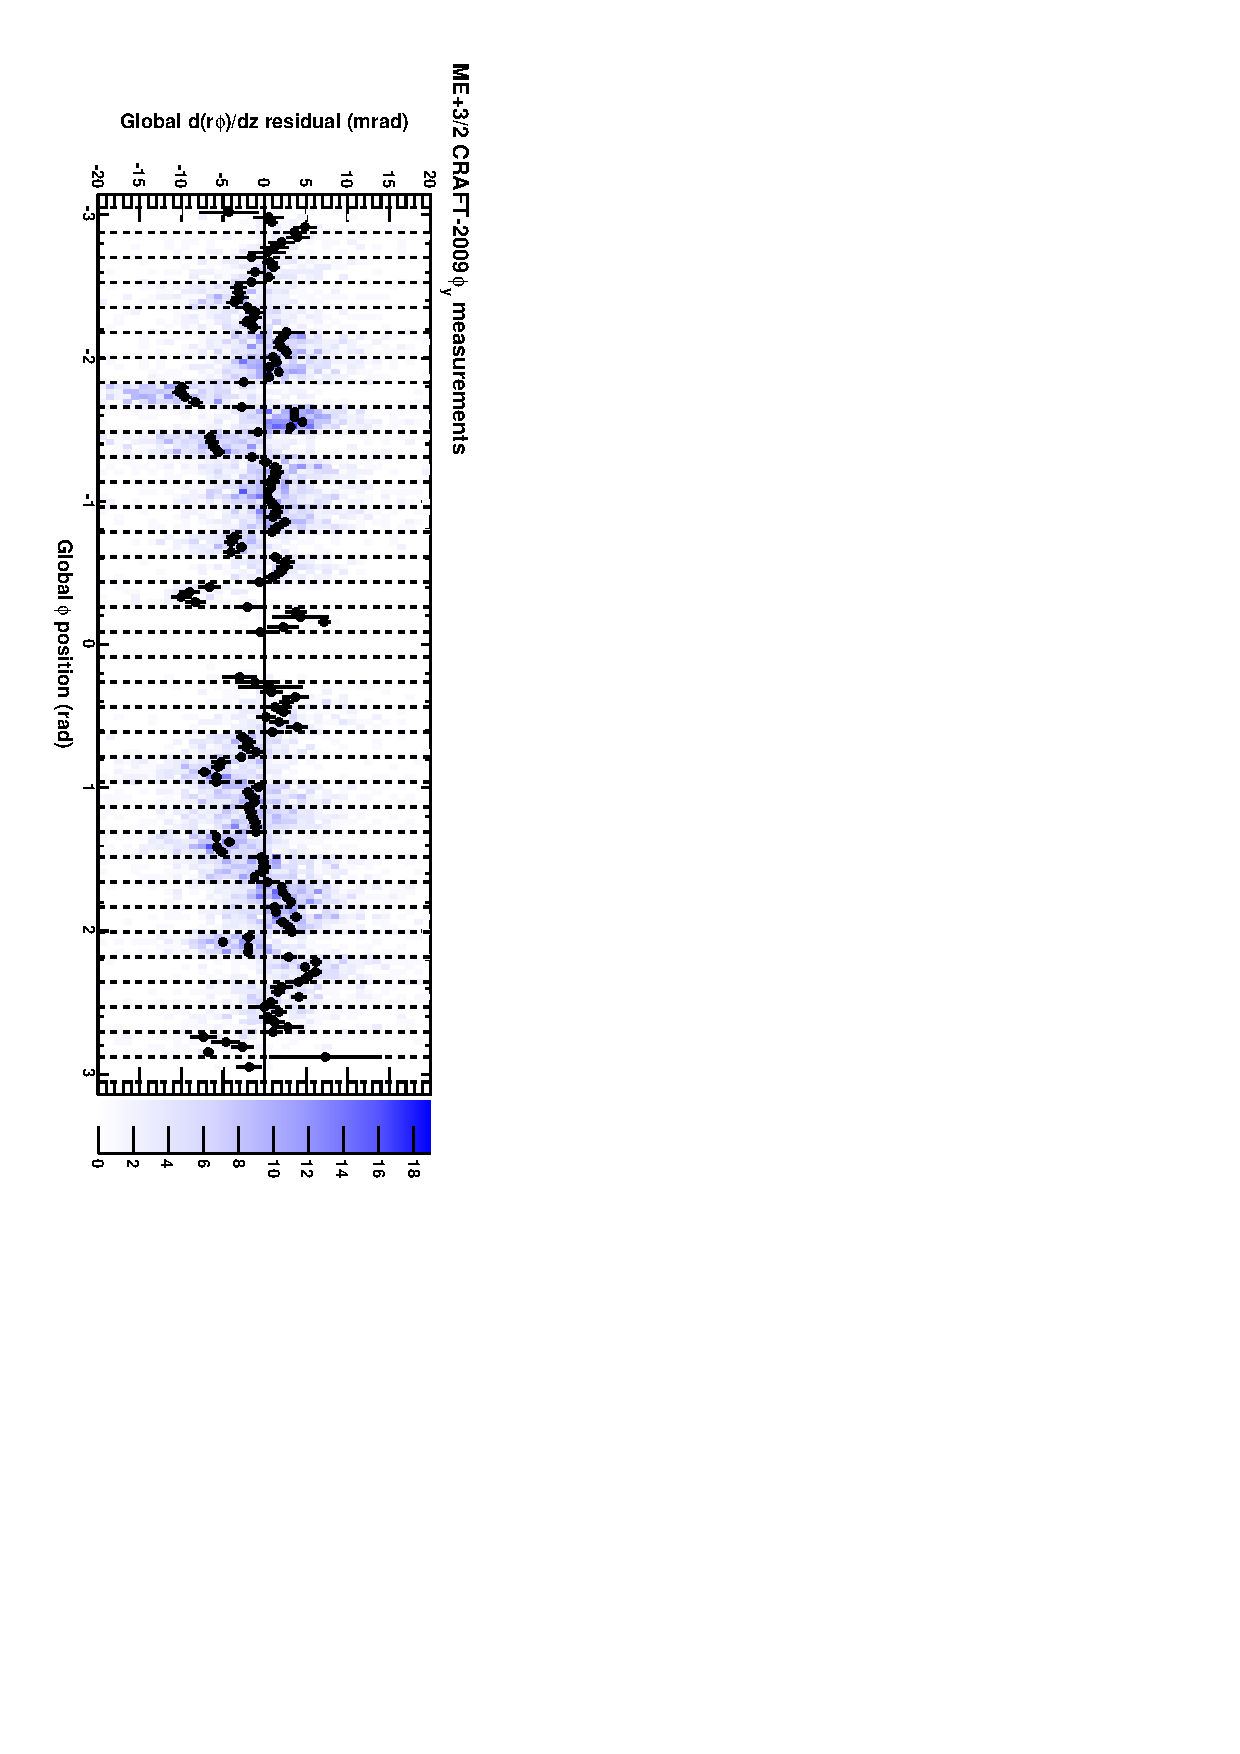
\includegraphics[height=\linewidth, angle=90]{correspondance_2009_mep32_phiy.pdf}
\end{frame}

\begin{frame}
\frametitle{Why?}
\framesubtitle{Why do we now have top-of-CMS hits on our globalMuons?}

\begin{itemize}
\item The cause has not been narrowed down: multiple changes

\begin{center}
\renewcommand{\arraystretch}{1.5}
\begin{tabular}{c | c}
{\bf old} & {\bf new} \\\hline
CRAFT-2008 & CRAFT-2009 \\
CMSSW\_2\_2\_11 & CMSSW\_3\_1\_2 \\
CSCSkim & prompt RECO \\
\end{tabular}
\end{center}

\item Common features:
\begin{itemize}
\item 100 $<$ $p_T$ $<$ 200~GeV (new to the analysis: not much is lost
  when also requiring high-quality oblique-angle tracks)
\item final CRAFT-2008 tracker alignment and APEs
\item most plots produced with DESIGN geometry
\end{itemize}

\item These are {\it not} bottom-only trigger data: 109459--111136
\item It is, of course a good thing: with this coverage, we should be
  able to reliably align disks (and many individual chambers)
\end{itemize}
\end{frame}

\begin{frame}
\frametitle{Agreement with beam-halo!}
\framesubtitle{Wider coverage allows us to see that the correlation is real}

\vspace{0.2 cm}
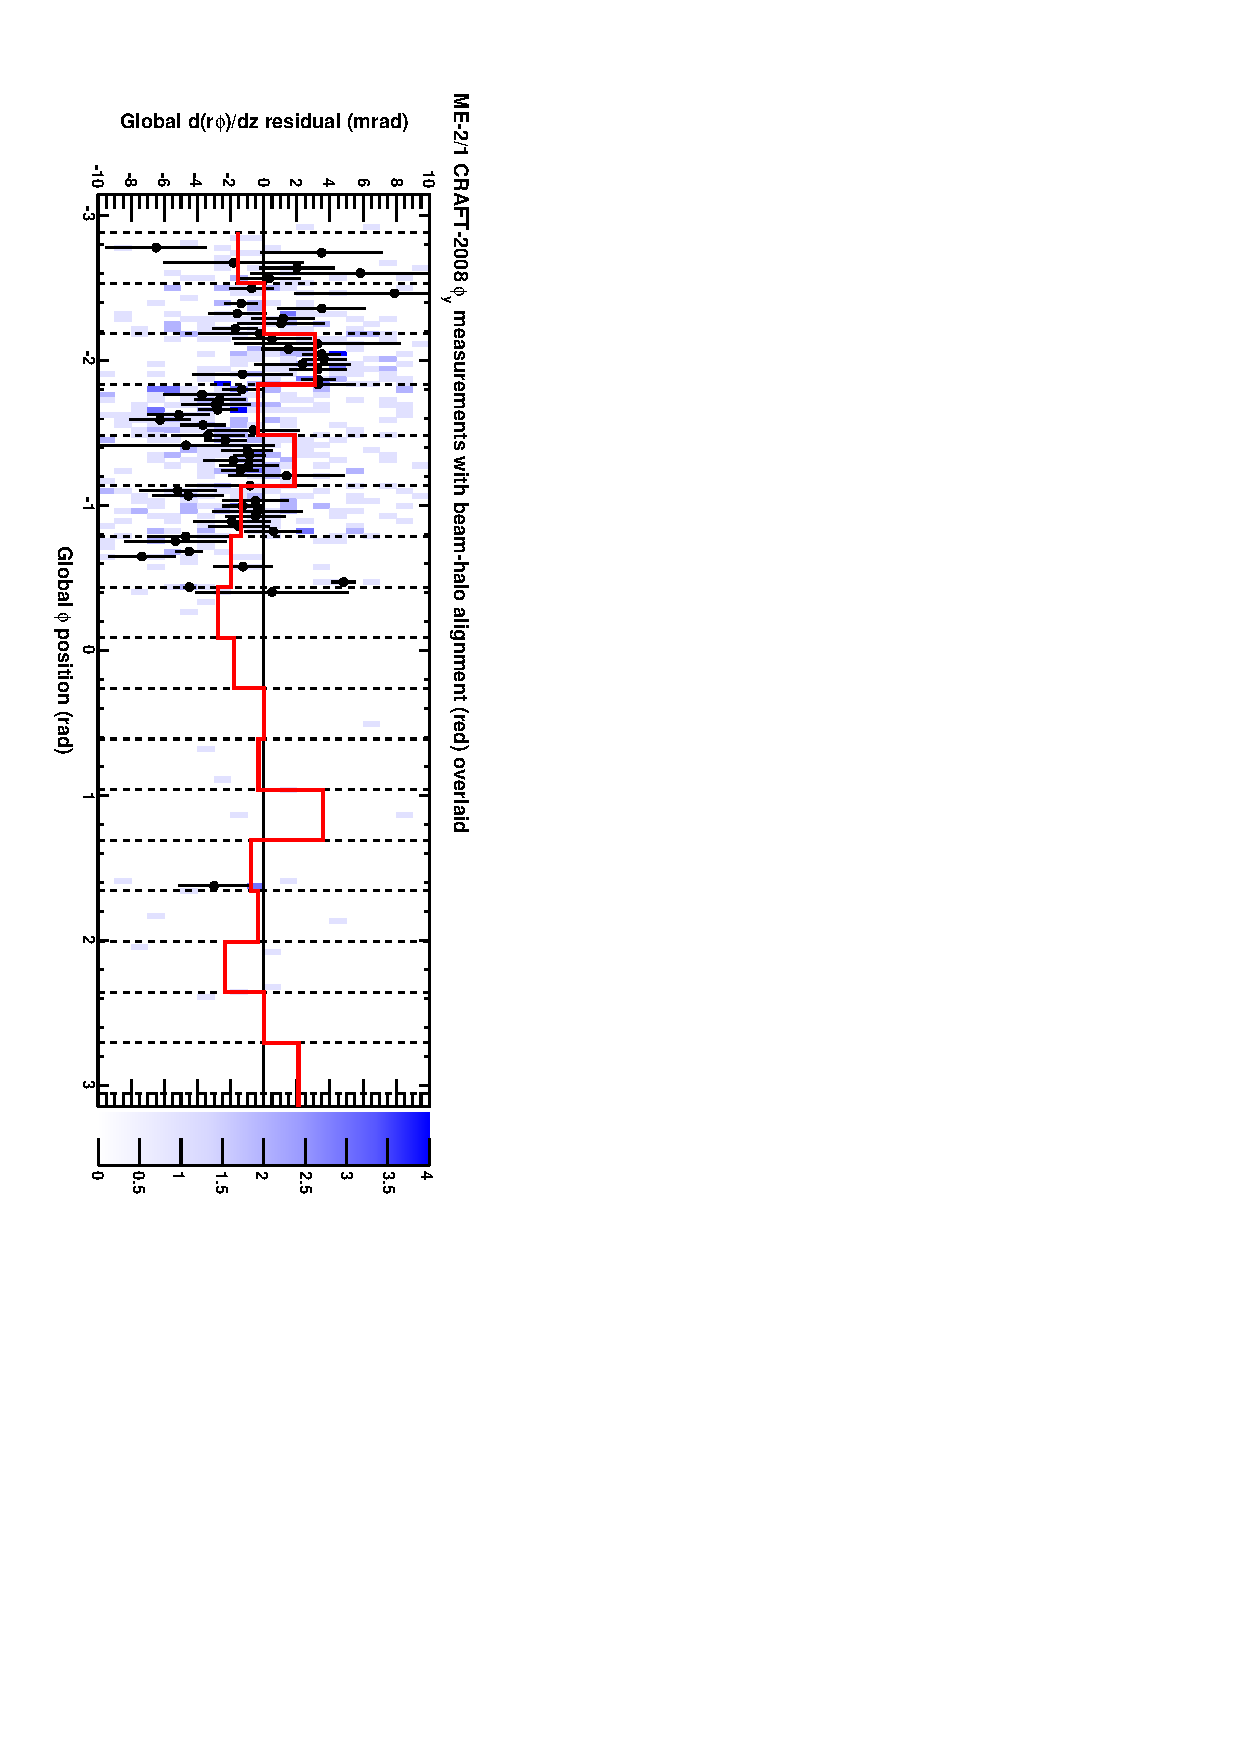
\includegraphics[height=\linewidth, angle=90]{beamhalo_2008_mem21.pdf}

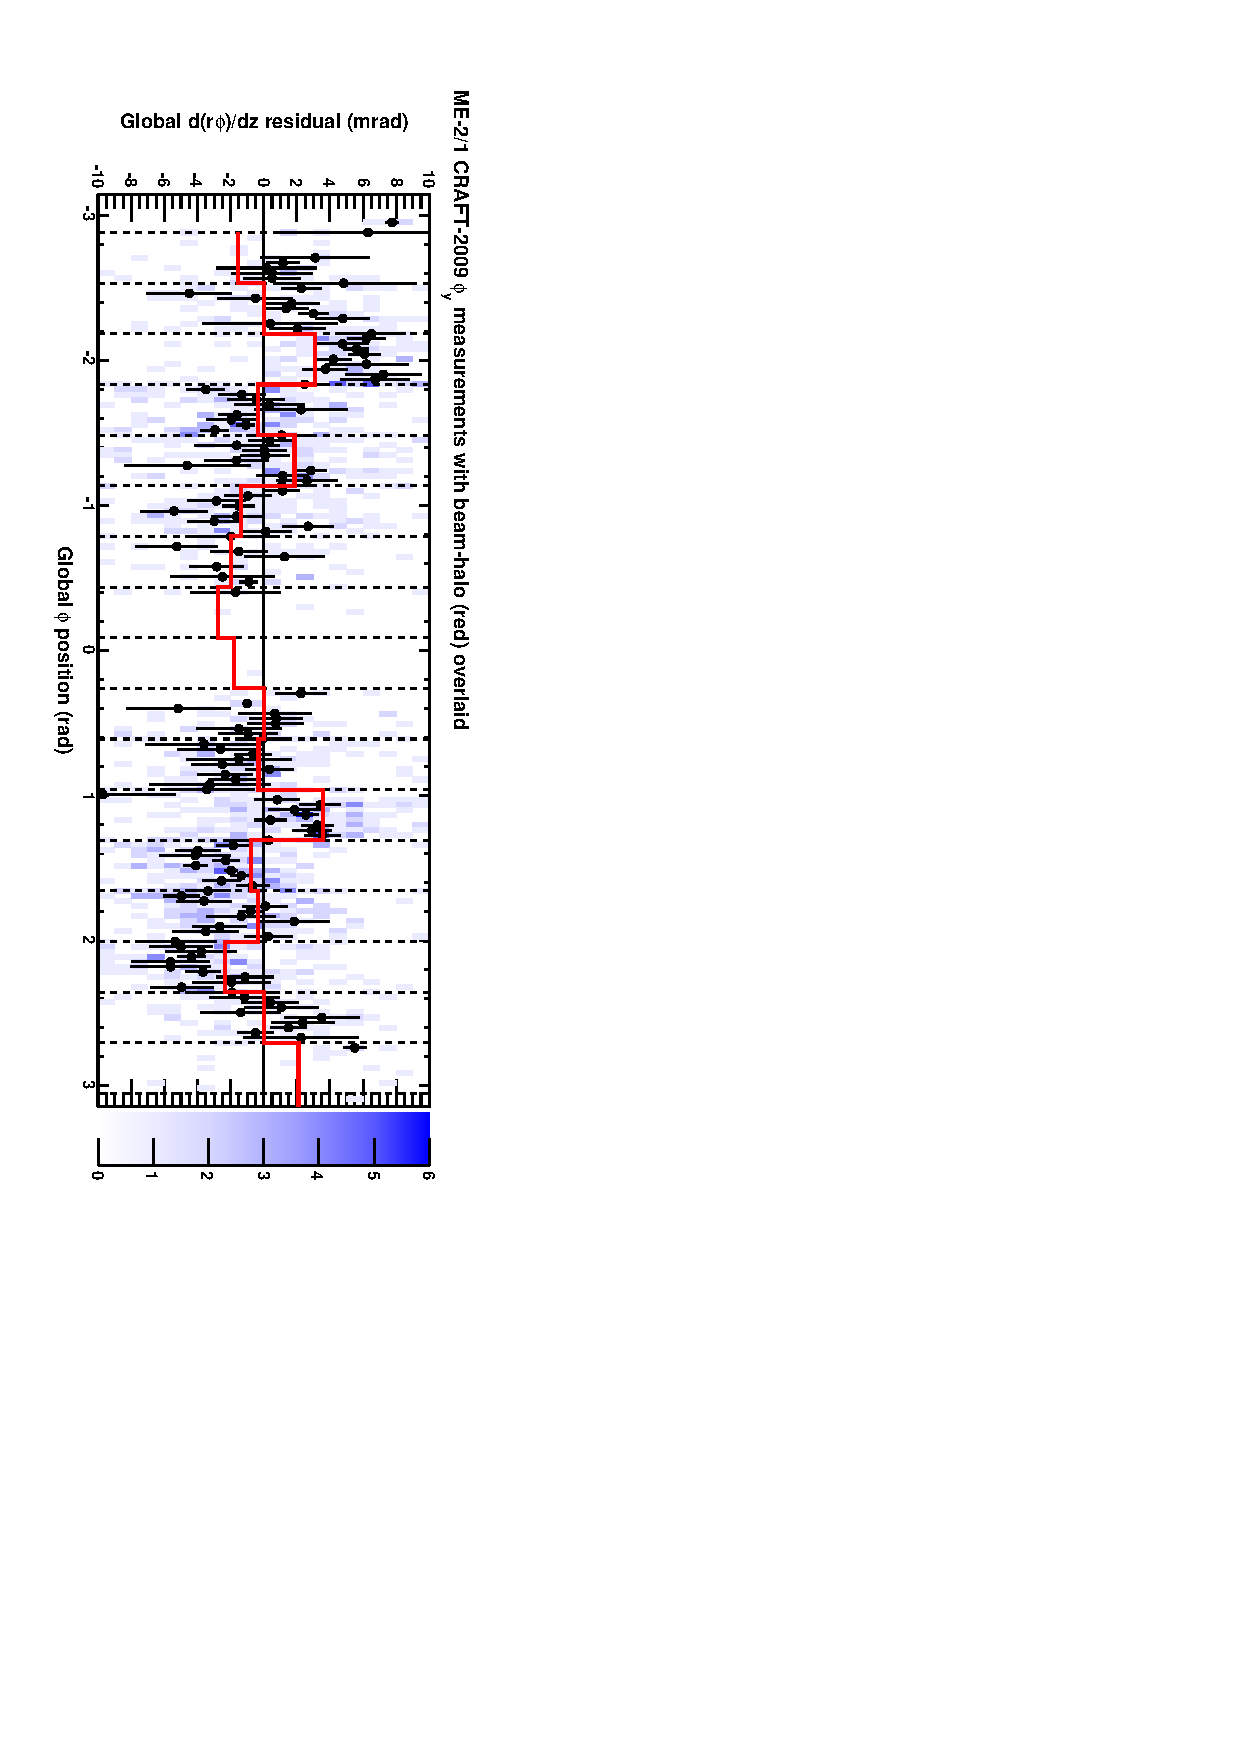
\includegraphics[height=\linewidth, angle=90]{beamhalo_2009_mem21.pdf}
\end{frame}

\begin{frame}
\frametitle{Agreement with beam-halo?}
\framesubtitle{But there are some significant differences: likely real motion}

\vspace{0.2 cm}
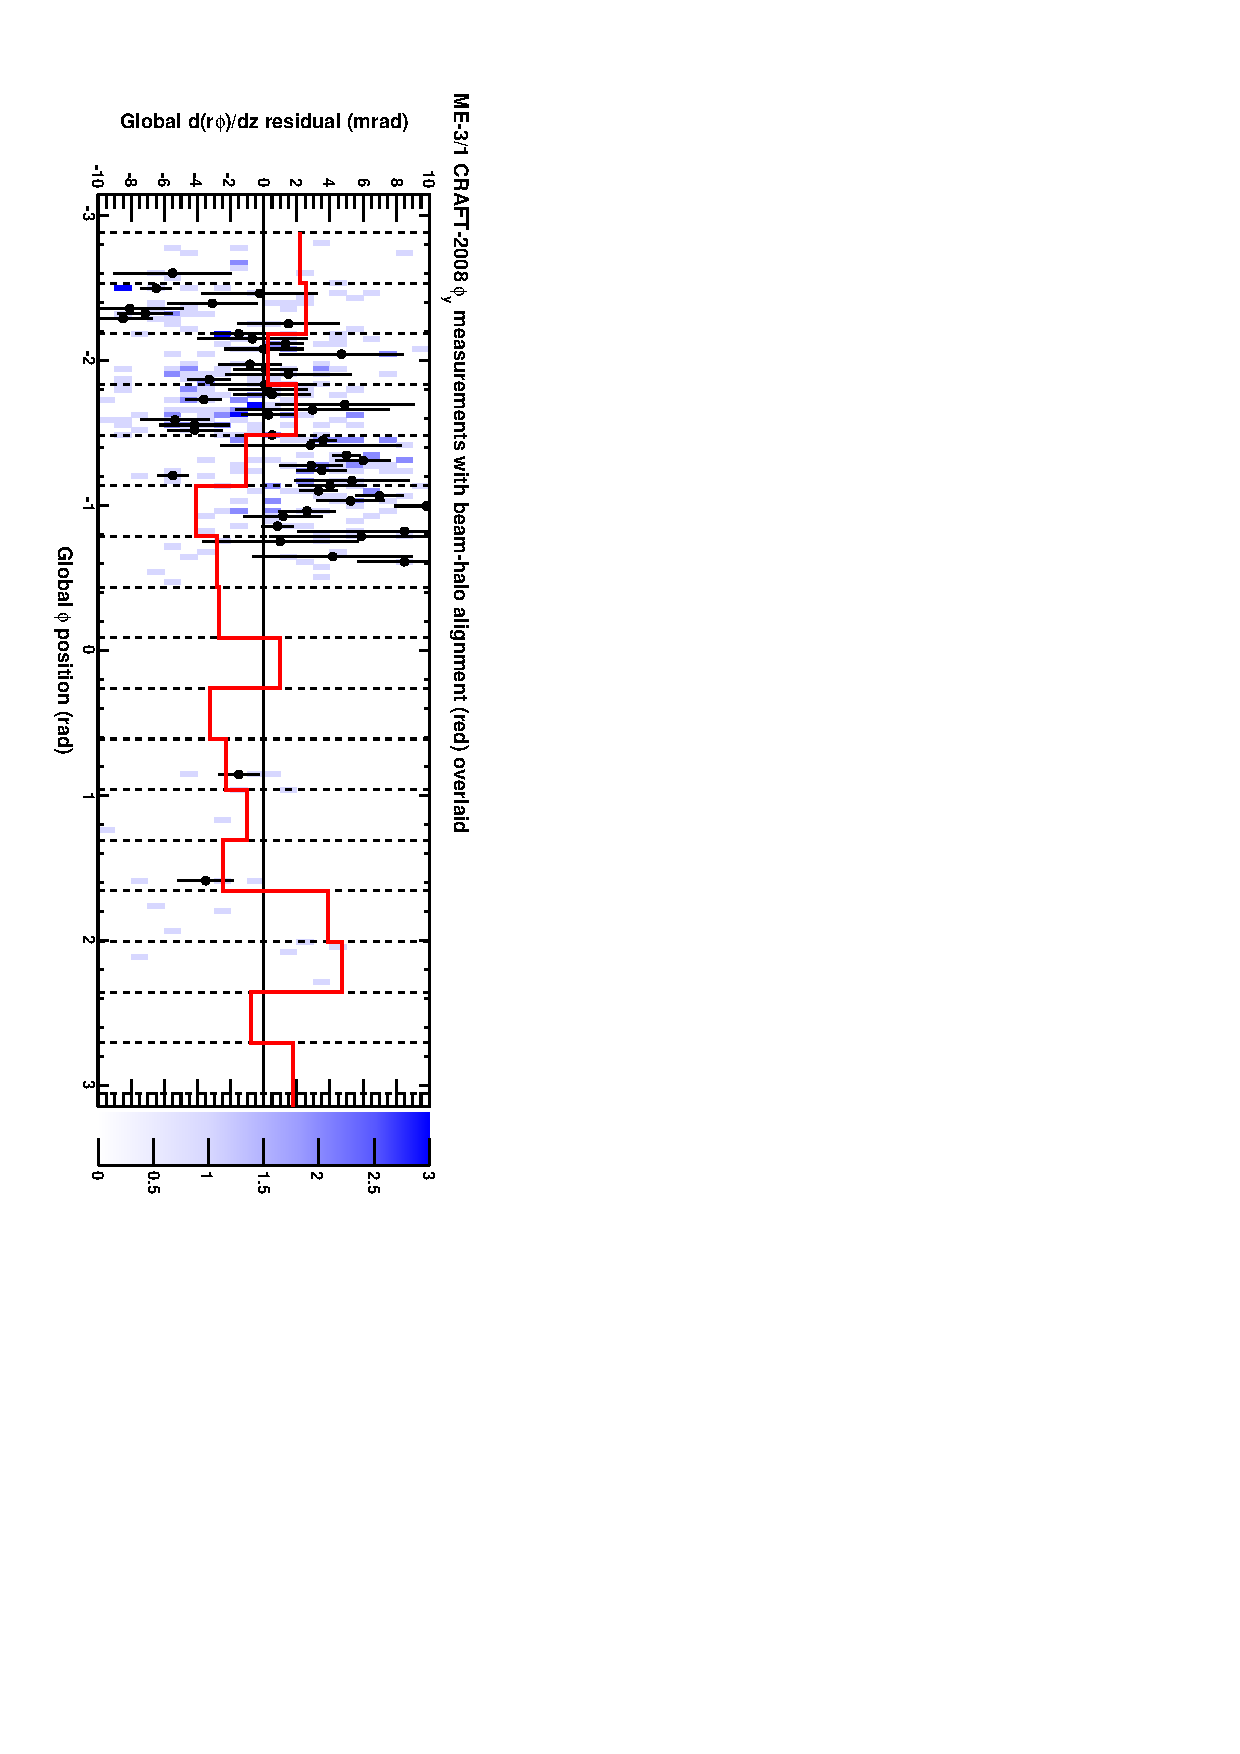
\includegraphics[height=\linewidth, angle=90]{beamhalo_2008_mem31.pdf}

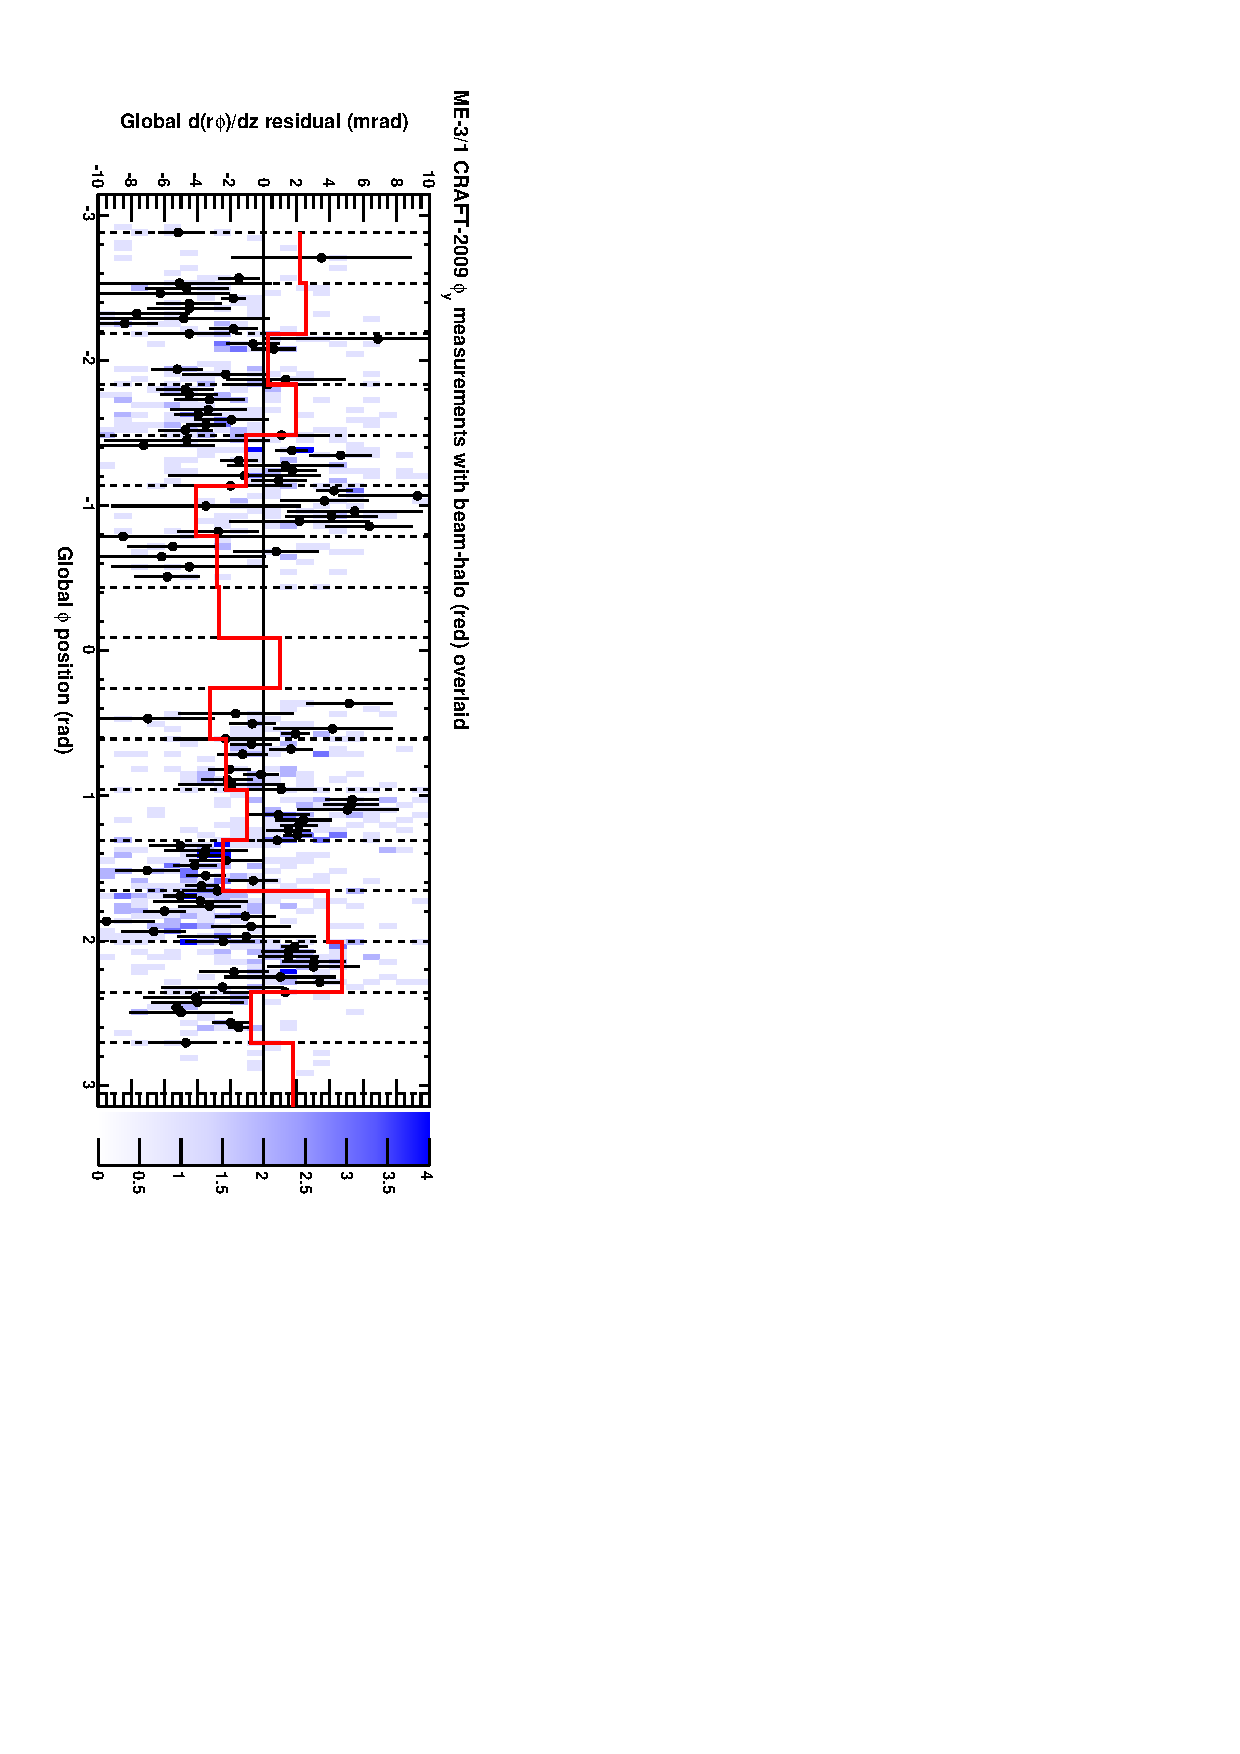
\includegraphics[height=\linewidth, angle=90]{beamhalo_2009_mem31.pdf}
\end{frame}

\begin{frame}
\begin{center}
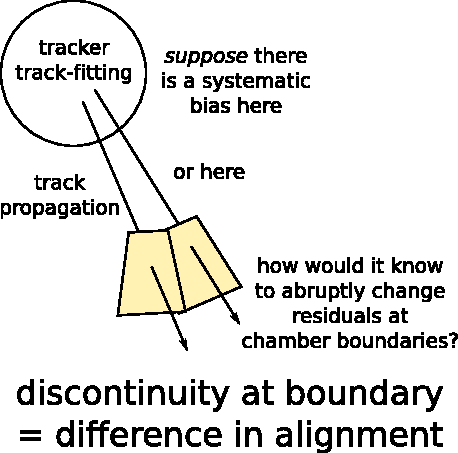
\includegraphics[width=0.6\linewidth]{argument.pdf}
\end{center}

\large \ldots or something else related to the chambers themselves, not the track source
\end{frame}

\begin{frame}
\frametitle{$\Delta r\phi$ position residuals}
\framesubtitle{Nicely completed $(\mbox{const} + \sin\phi + \cos\phi)$ curve, but why the alteration?}

\vspace{0.2 cm}
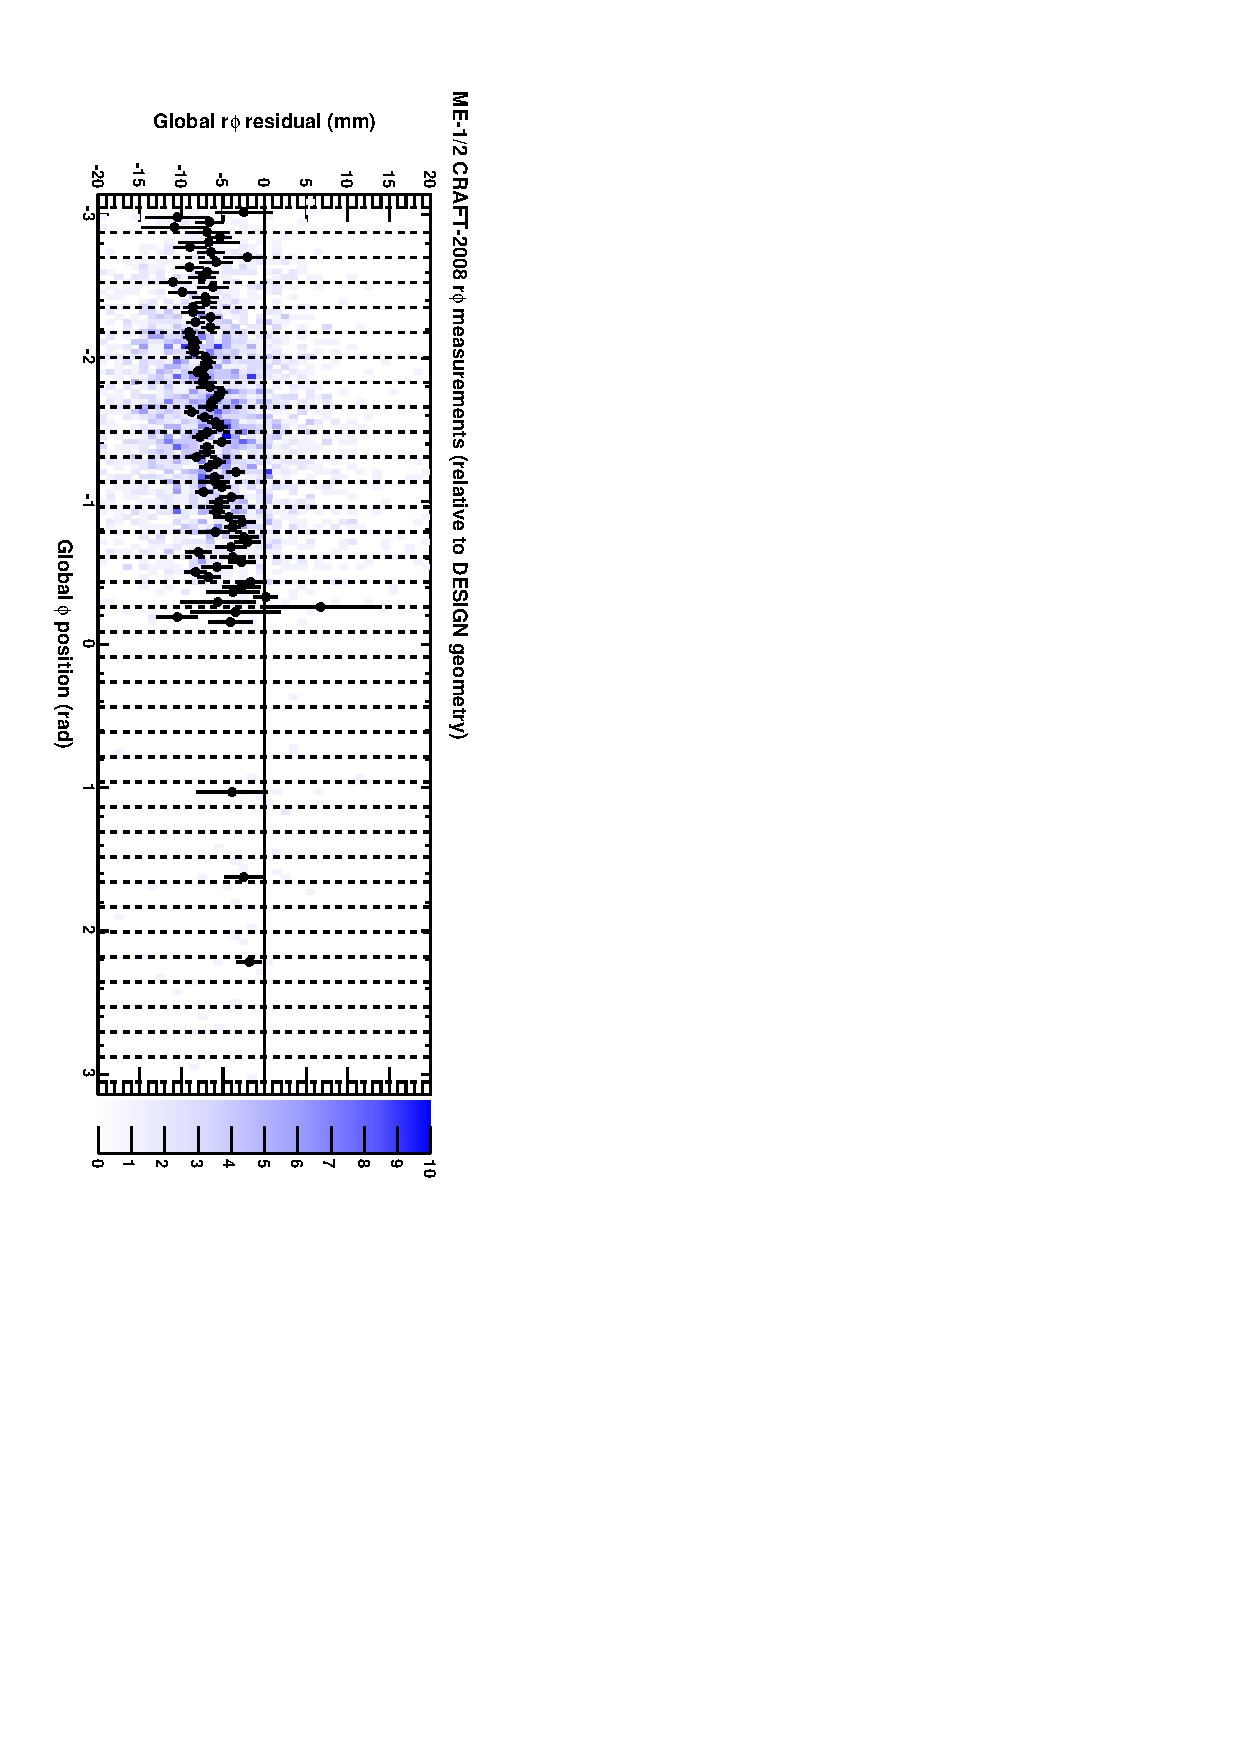
\includegraphics[height=\linewidth, angle=90]{alternation_2008_mem12_design.pdf}

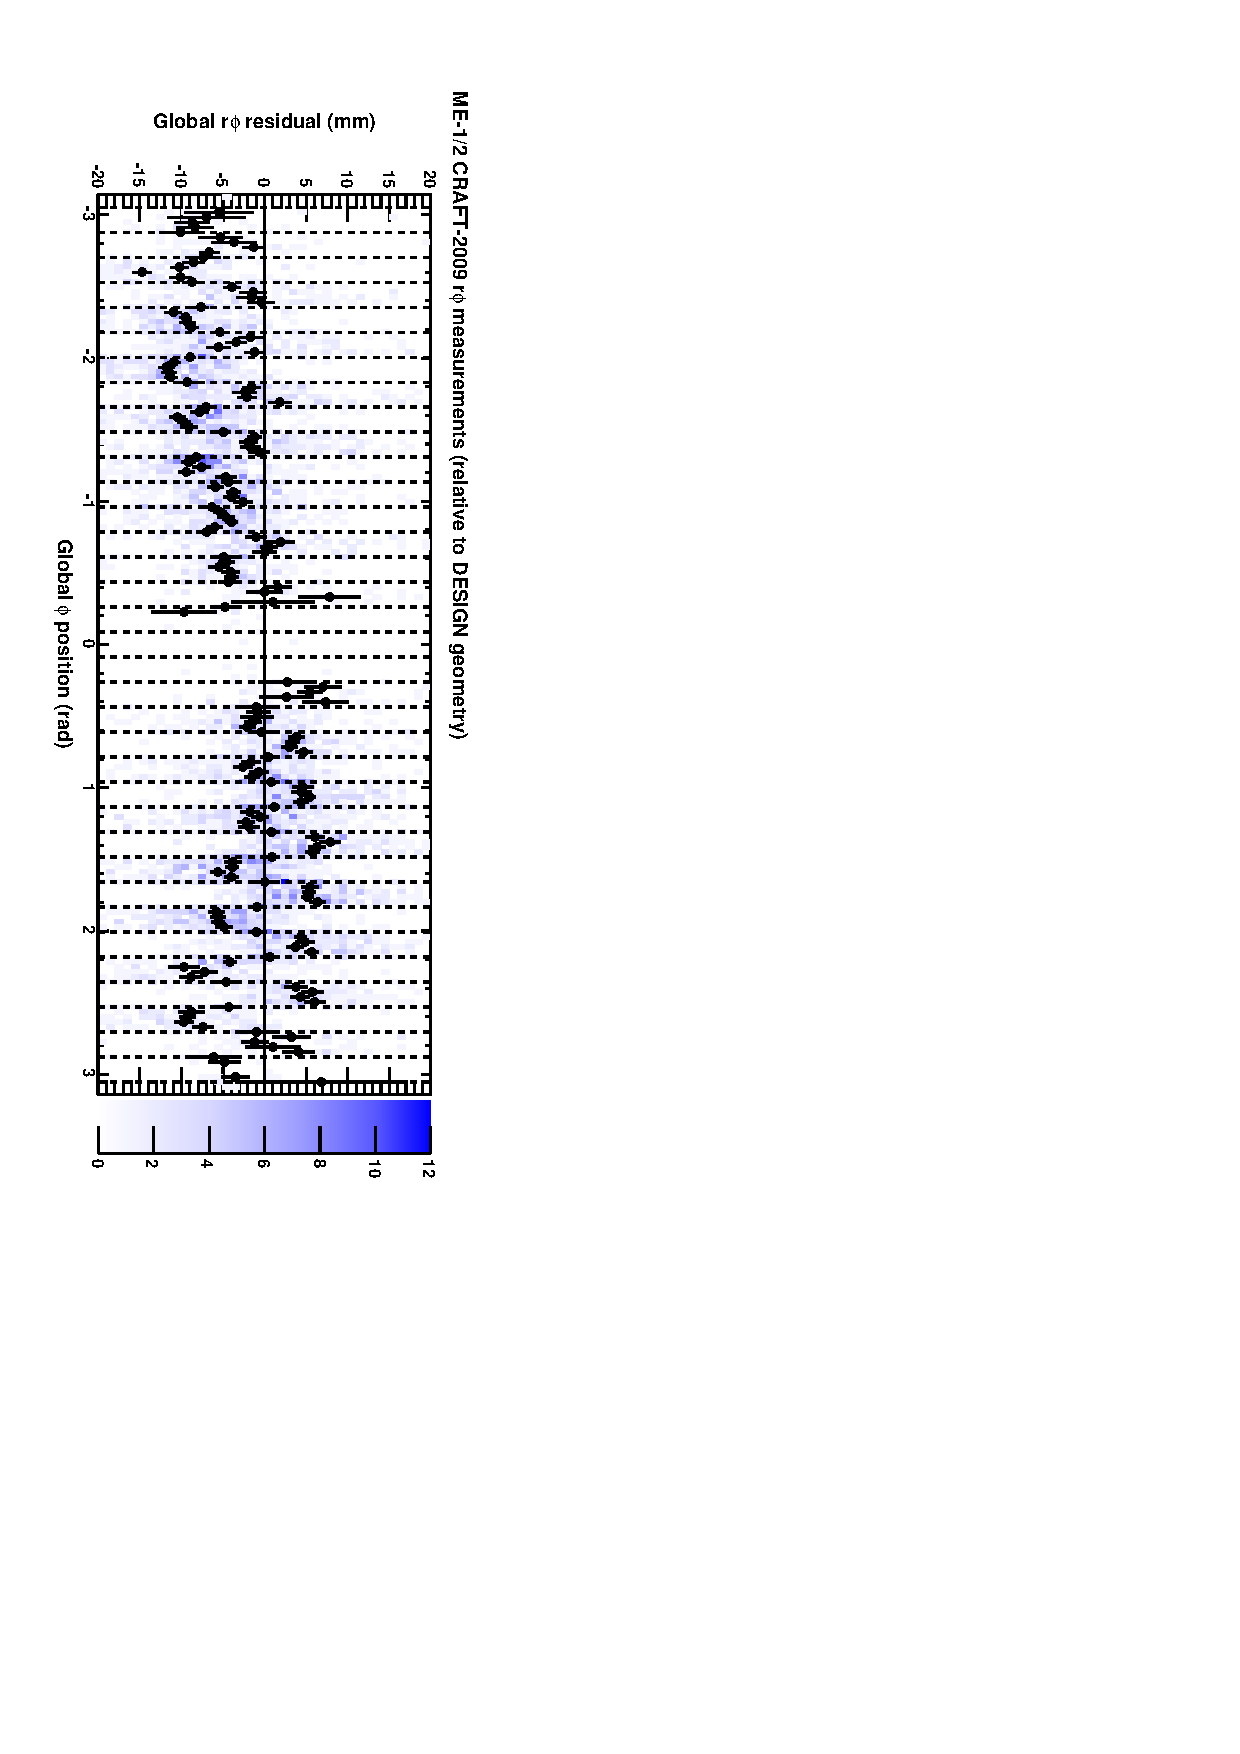
\includegraphics[height=\linewidth, angle=90]{alternation_2009_mem12_design.pdf}
\end{frame}

\begin{frame}
\frametitle{Now with HW/PG geometry\ldots}
\framesubtitle{Also insensitive to a 1~cm translation in $z$}

\vspace{0.2 cm}
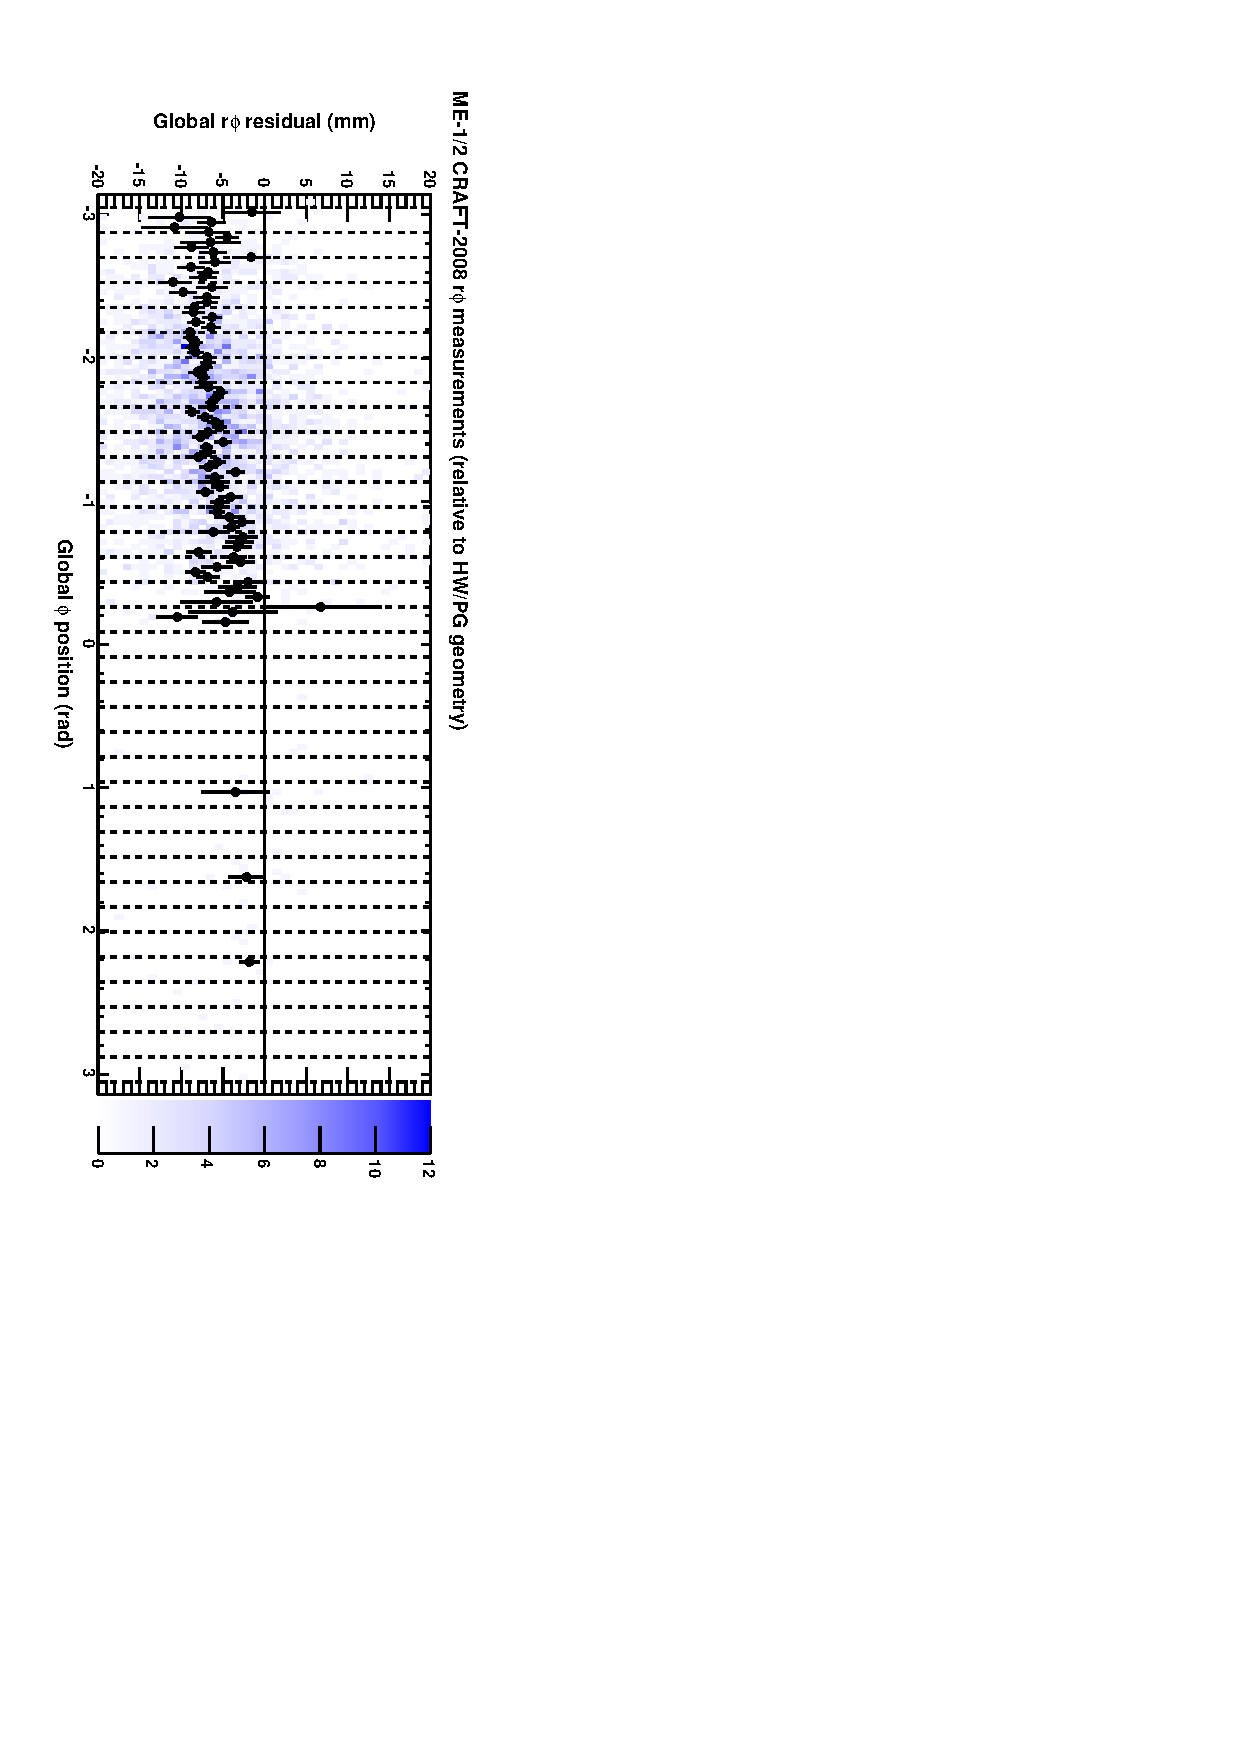
\includegraphics[height=\linewidth, angle=90]{alternation_2008_mem12_hwpg.pdf}

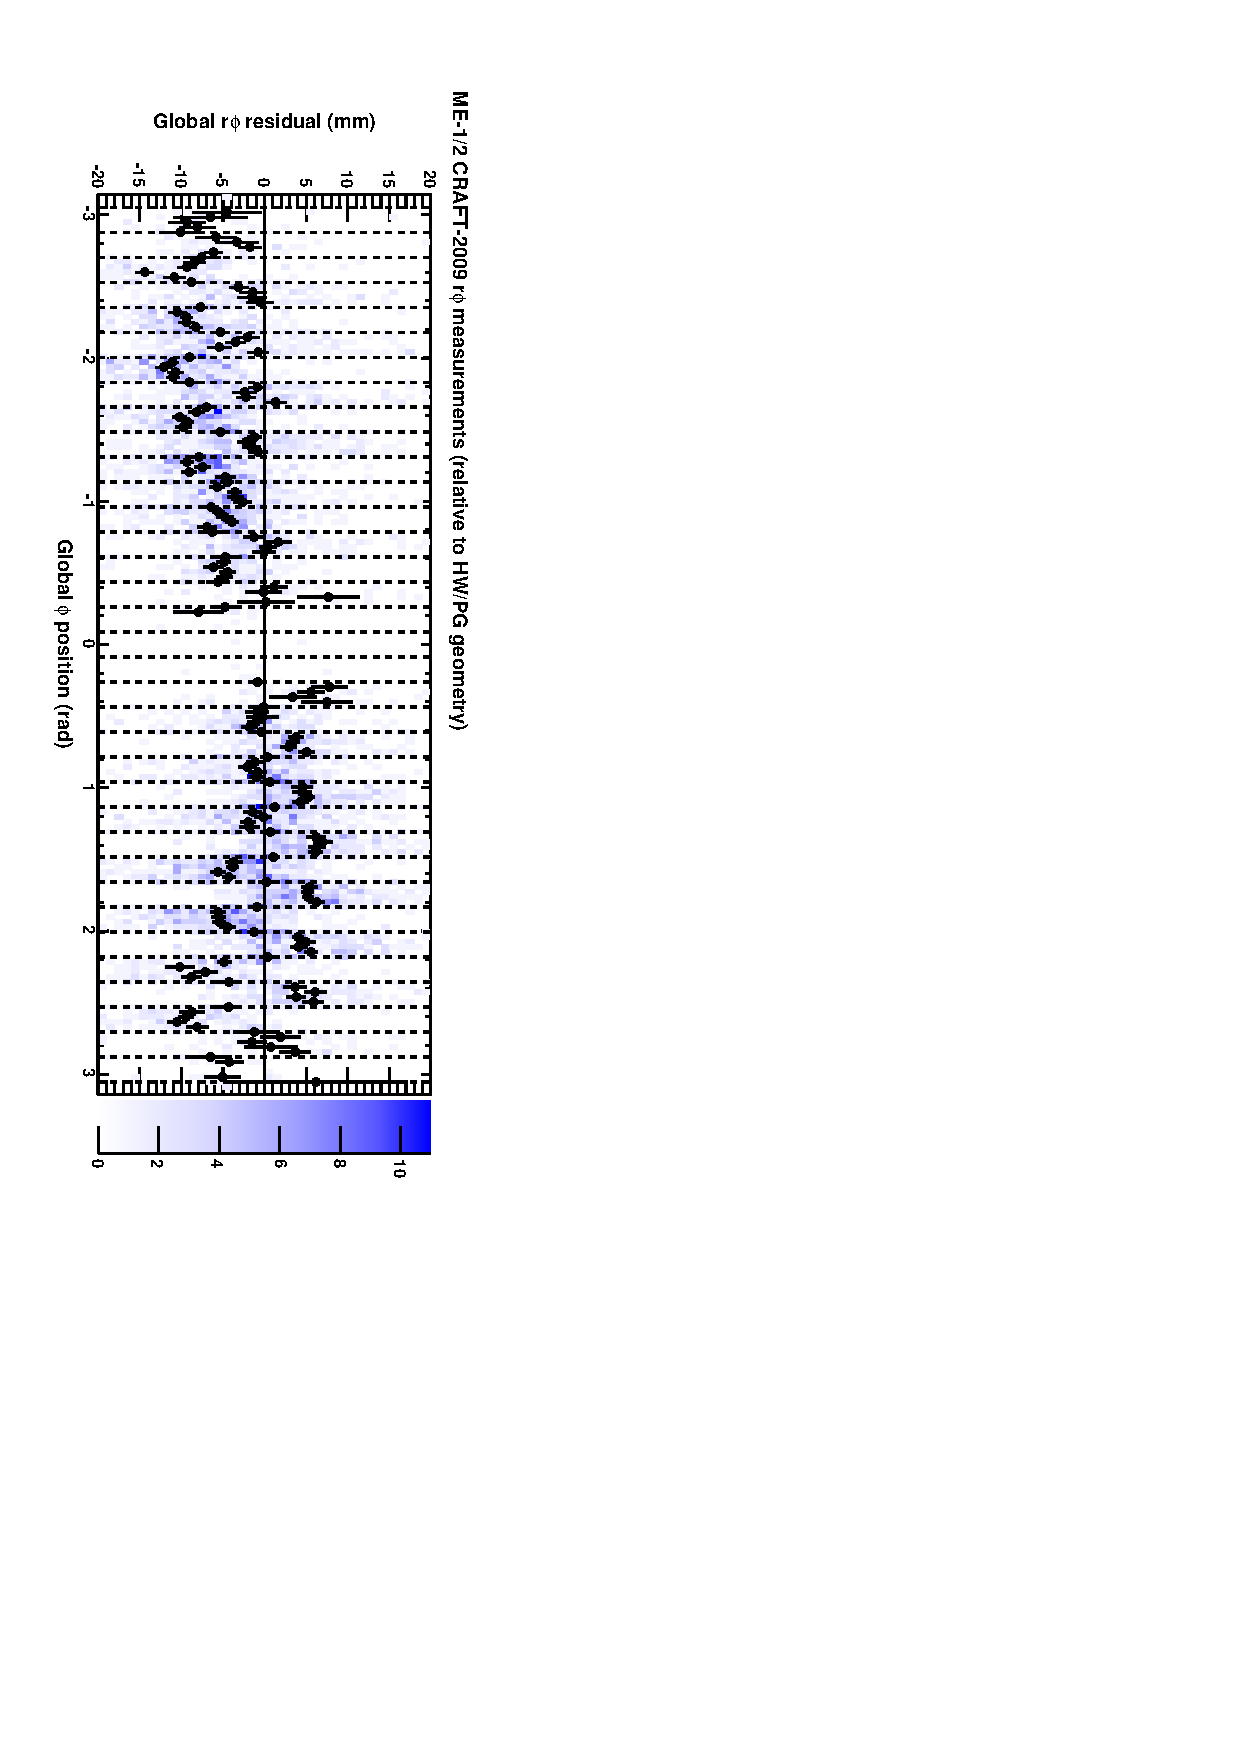
\includegraphics[height=\linewidth, angle=90]{alternation_2009_mem12_hwpg.pdf}
\end{frame}

\begin{frame}
\frametitle{The other projection}
\framesubtitle{Selected two neighboring chambers and plot vs.~$R$; nothing strange}

\vspace{0.2 cm}
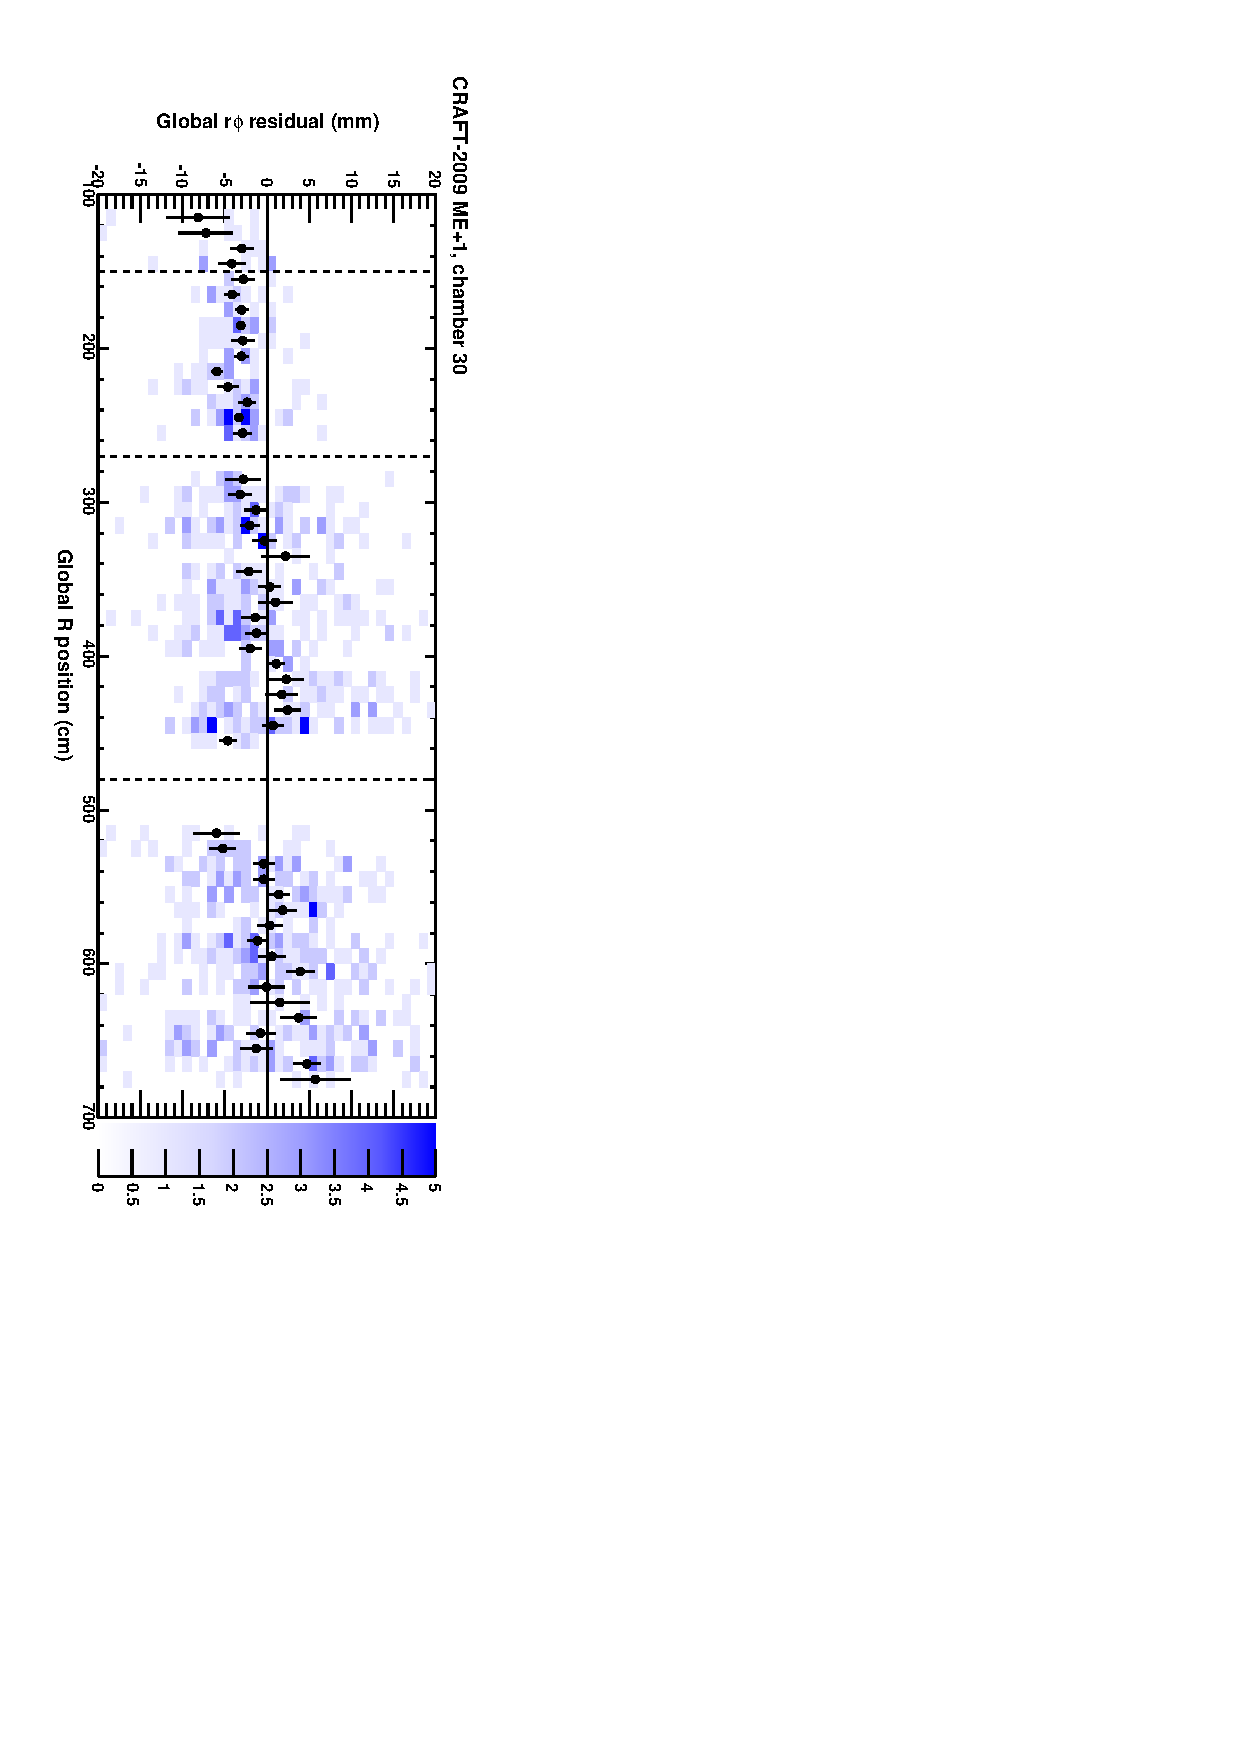
\includegraphics[height=\linewidth, angle=90]{alternation_2009-30.pdf}

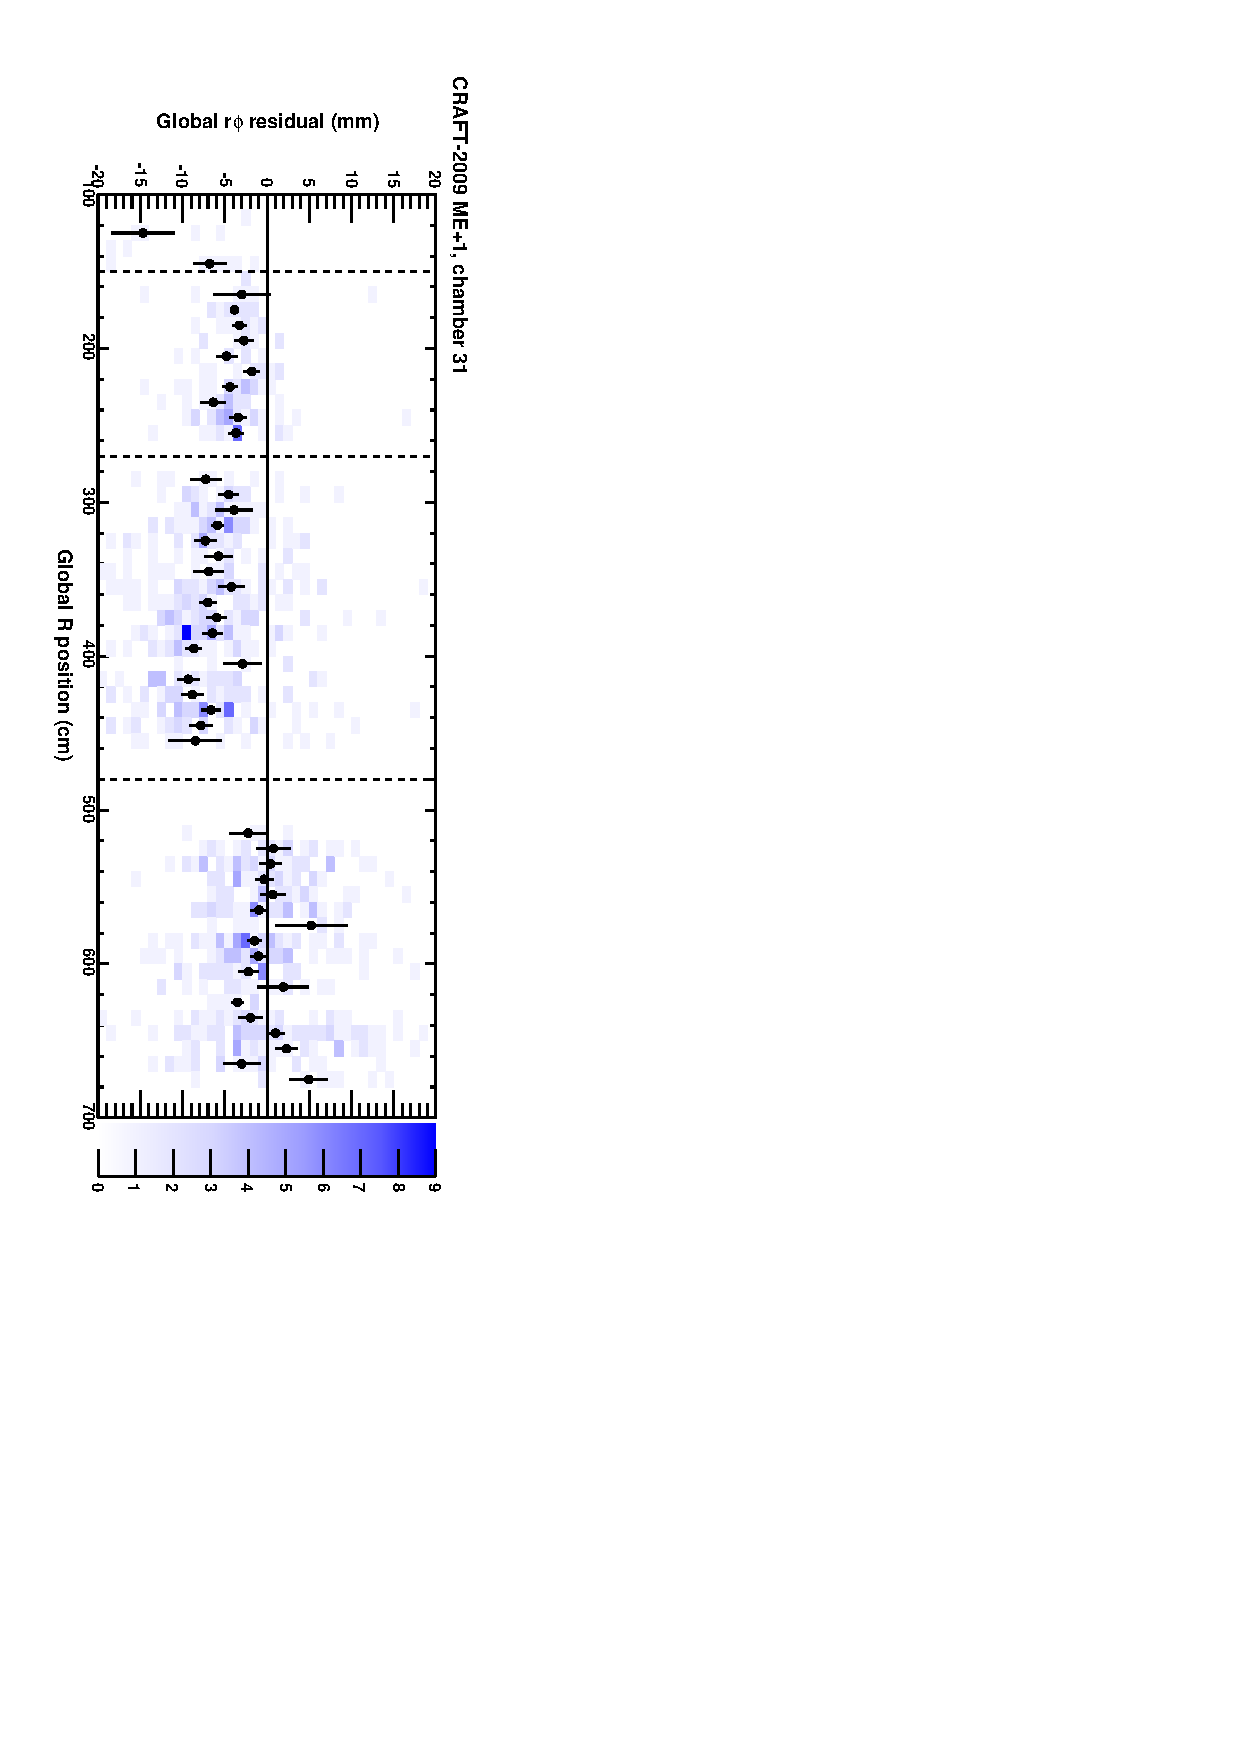
\includegraphics[height=\linewidth, angle=90]{alternation_2009-31.pdf}
\end{frame}

\begin{frame}
\frametitle{Summary of alteration pattern}

\begin{itemize}\setlength{\itemsep}{0.25 cm}
\item Only affects ME$\pm x$/2.  ME$\pm x$/1 look fine and ME$\pm$1/3
  has a pattern all of its own.
\item Complete set of $\Delta r\phi$ vs.~$\phi$ in backup at the end of this talk
\item Are even-numbered chambers mechanically connected to each other
  in a different way from odd-numbered chambers?  Could a real motion
  like this have been physically introduced?

(I wouldn't think so)
\item Reconstruction bug?  Has something to do with local
  reconstruction or the local $\to$ global coordinate transformation\ldots
\begin{itemize}
\item alignment residuals constructed from CSCRecHit2Ds
\item same plotting code: only CMSSW version and primary dataset changed (see p.~5)
\end{itemize}

\item Apart from this, we're in a position to do a high-quality disk alignment
(unlike CRAFT-2008)
\end{itemize}
\end{frame}

\begin{frame}
\frametitle{Alignment of ME$+$4/2?}
\framesubtitle{They exist and are not obviously misaligned; not clear if they alternate}

\vspace{0.2 cm}
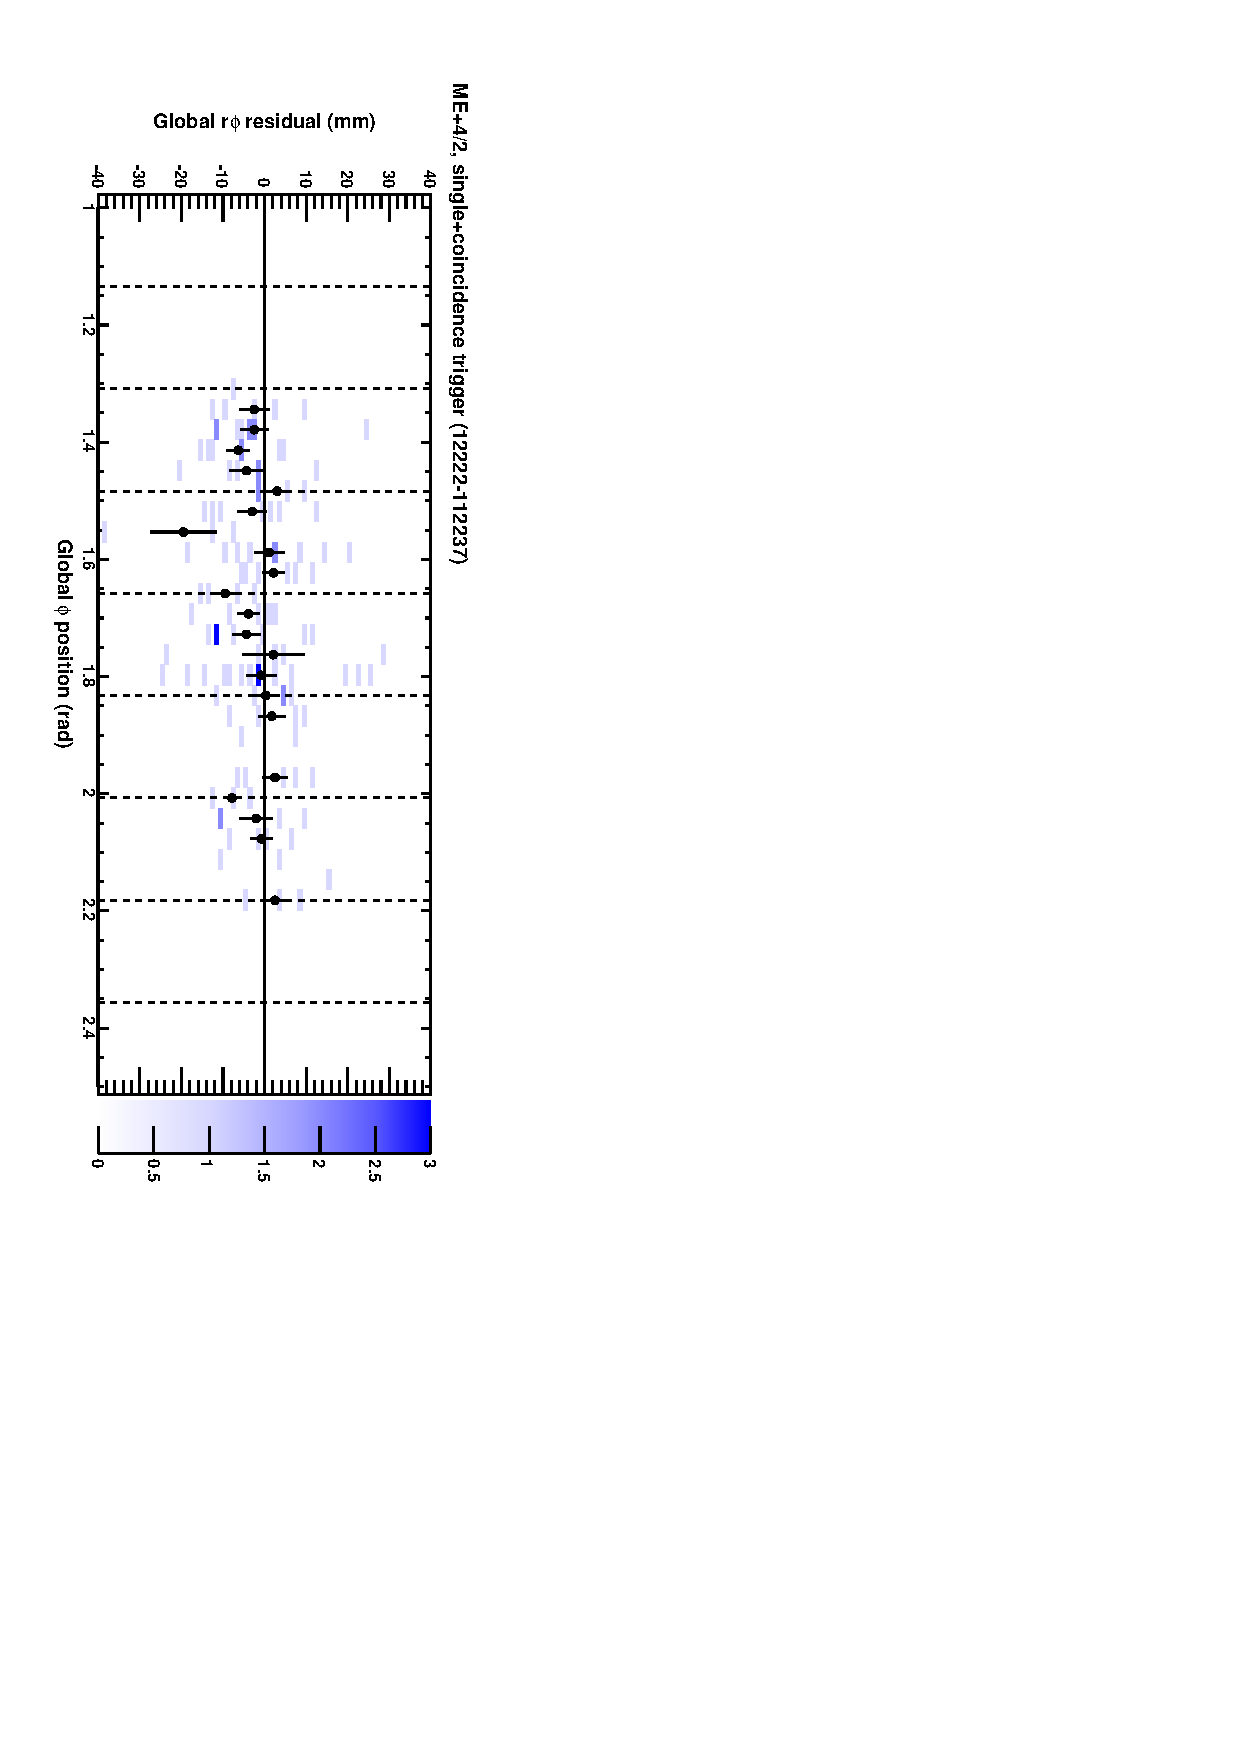
\includegraphics[height=\linewidth, angle=90]{mep42_singcoin.pdf}

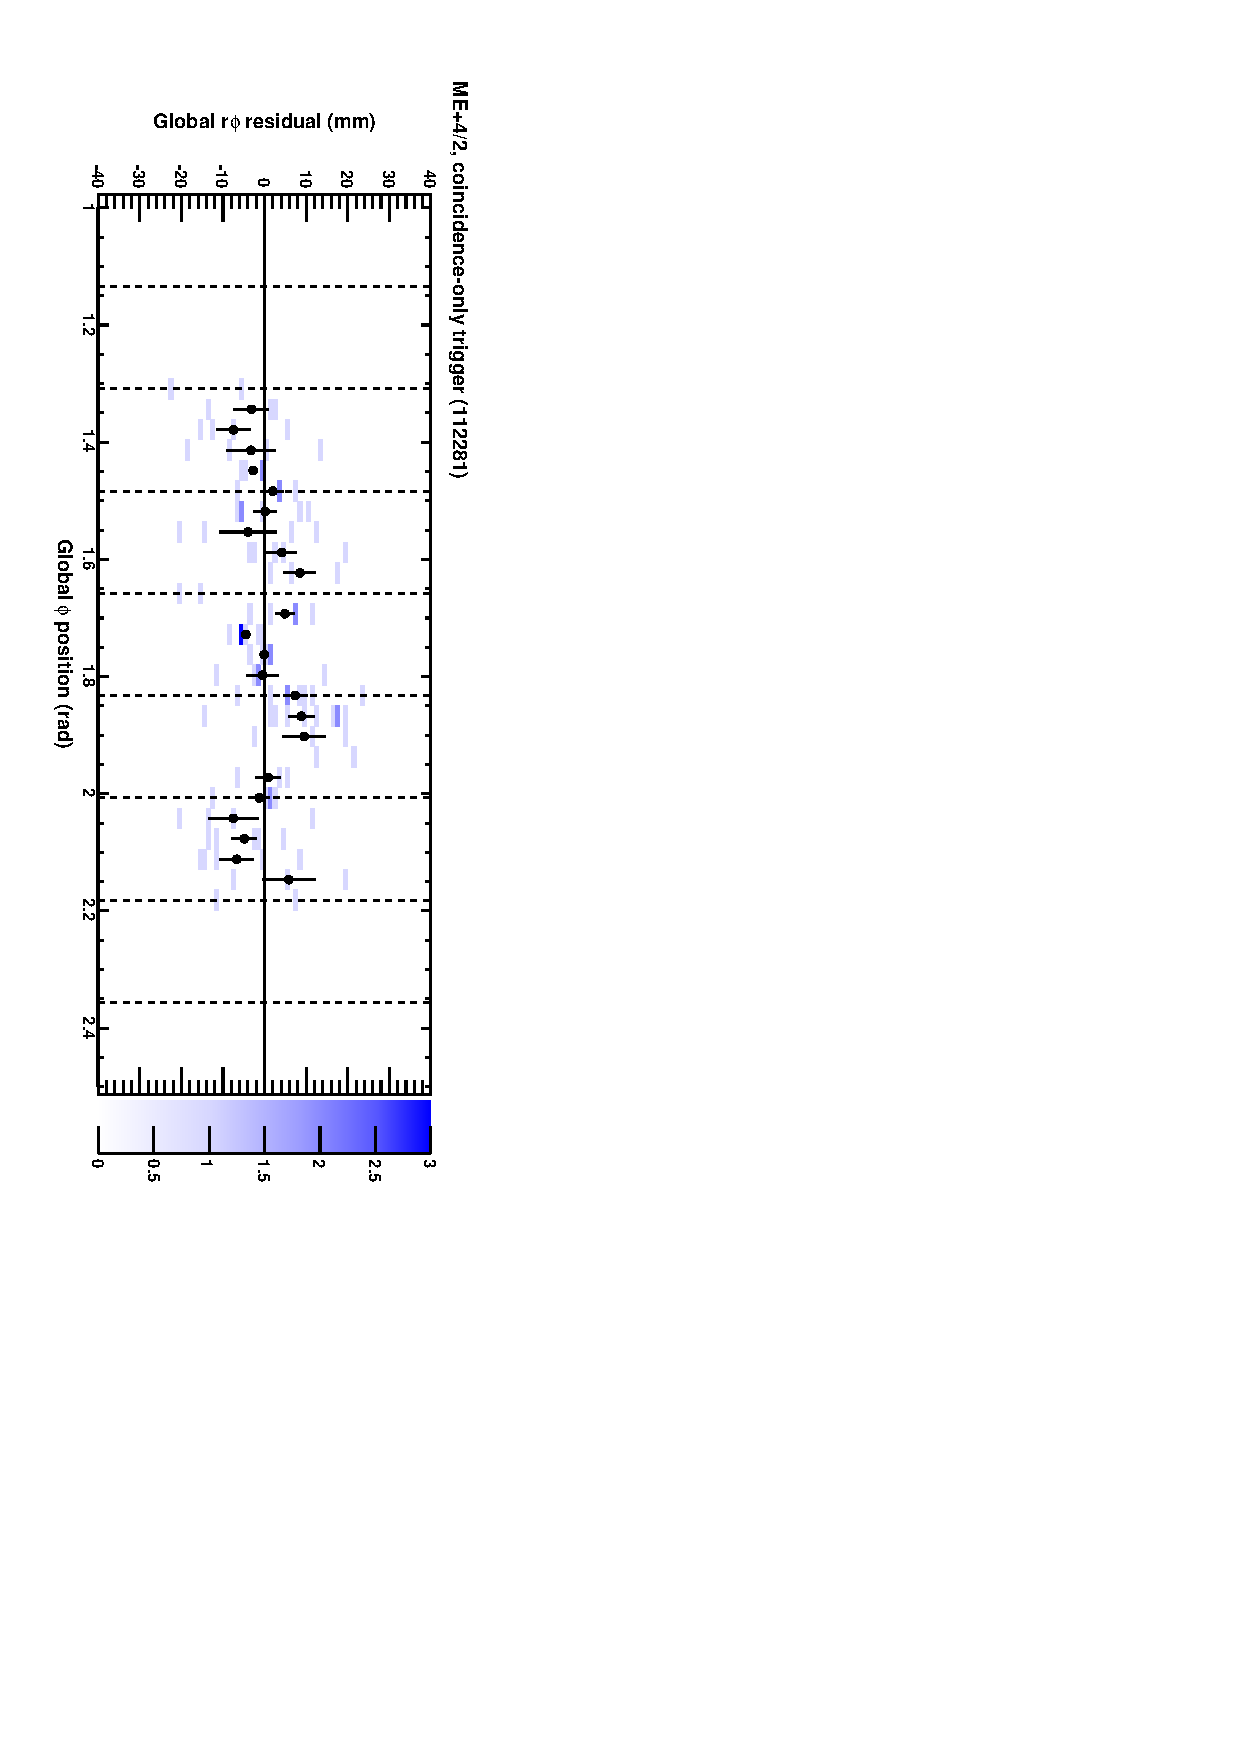
\includegraphics[height=\linewidth, angle=90]{mep42_coinonly.pdf}
\end{frame}

%% \section*{First section}
%% \begin{frame}
%% \begin{center}
%% \Huge \textcolor{blue}{First section}
%% \end{center}
%% \end{frame}

\begin{frame}
\frametitle{Summary}

\begin{itemize}\setlength{\itemsep}{0.25 cm}
\item CRAFT-2009 dataset provides more complete coverage in $\phi$, making it possible to do a real alignment
\item Reason for improved coverage is unknown
\item Can cross-check beam-halo $\phi_y$ measurements for the first
  time (photogrammetry could only cross-check $r\phi$ and $\phi_z$)
\item Likely that some $\phi_y$ angles changed by a few mrad in the past year
\item $r\phi$ residuals vs.~$\phi$ show clear $(\mbox{const} +
  \sin\phi + \cos\phi)$ curves (disk displacement and rotation), with
  a 1~cm alternation pattern superimposed
\item Reason for alternation is unknown
\end{itemize}

\label{numpages}
\end{frame}

\begin{frame}
\vspace{1 cm}
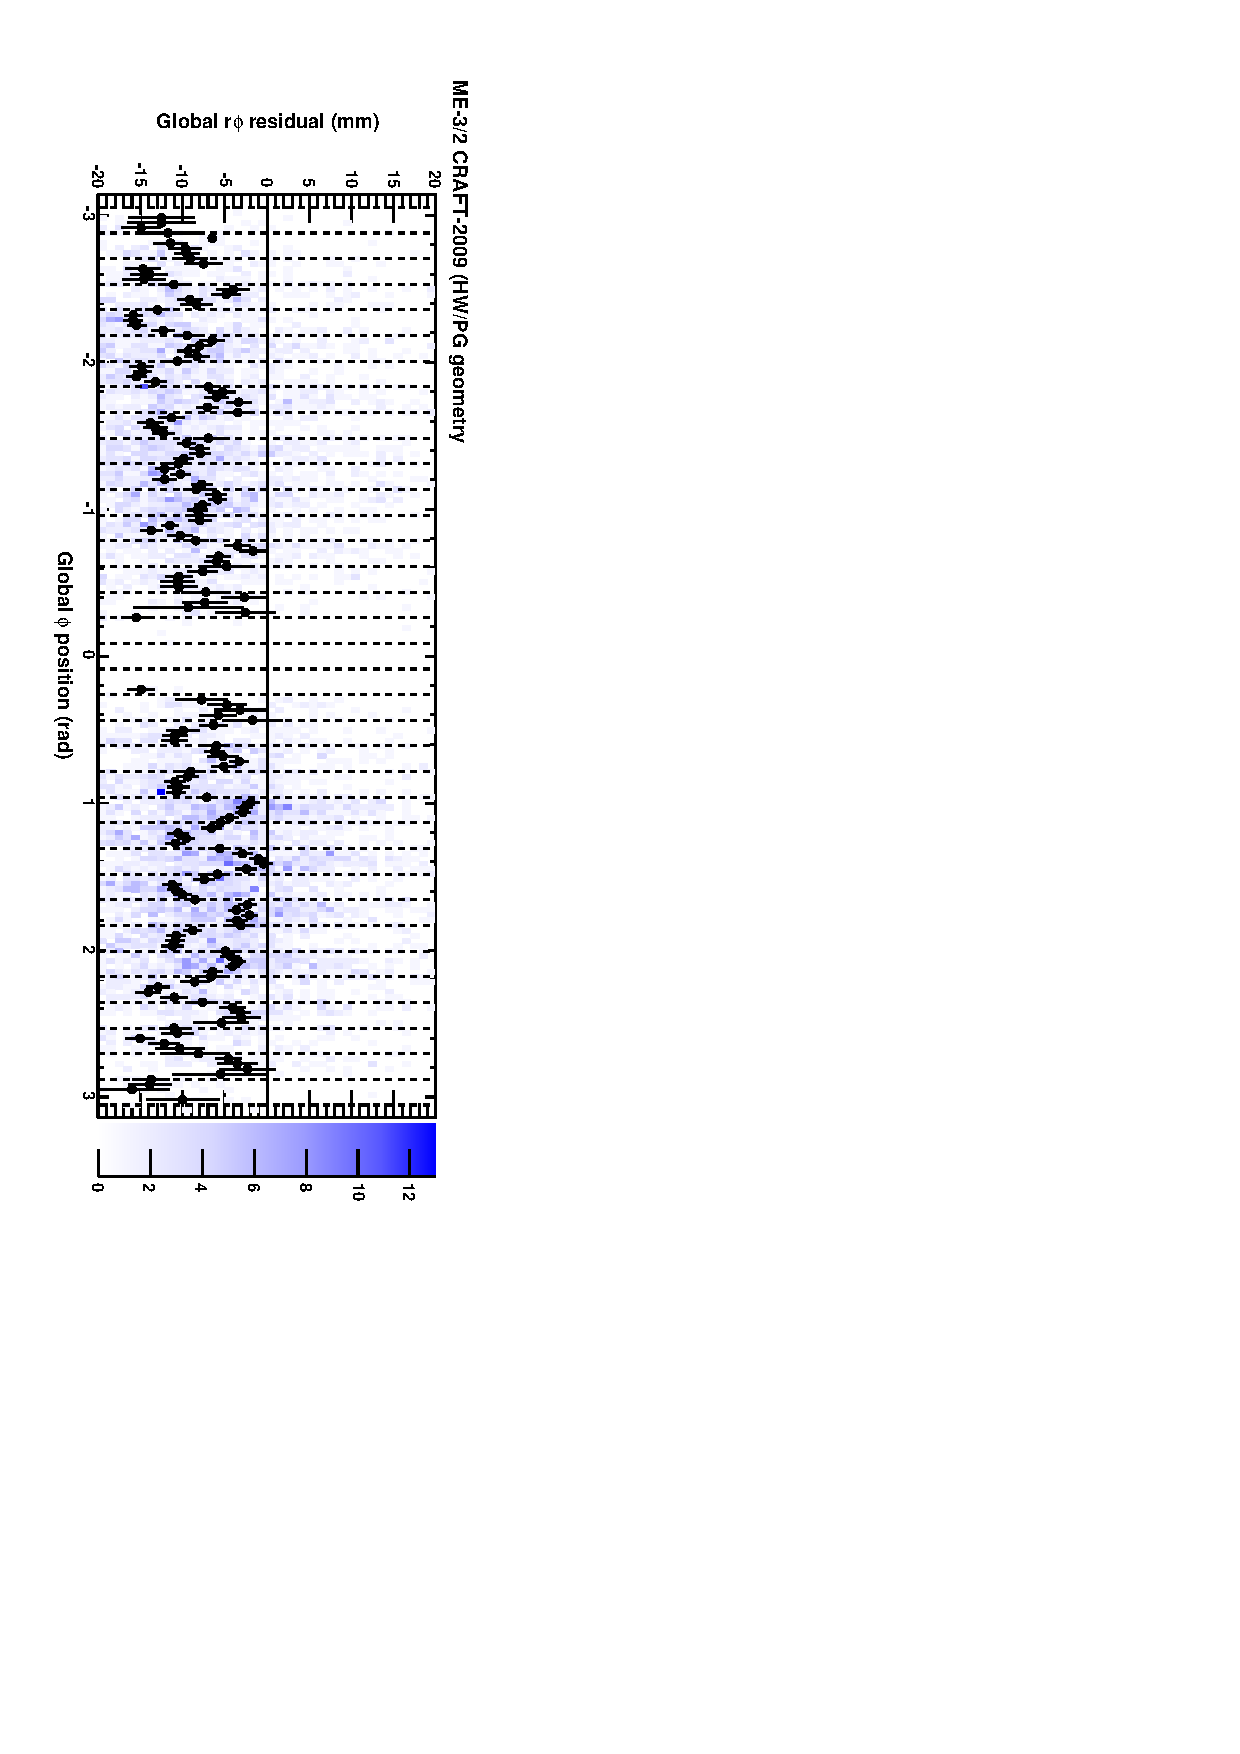
\includegraphics[height=\linewidth, angle=90]{series01.pdf}

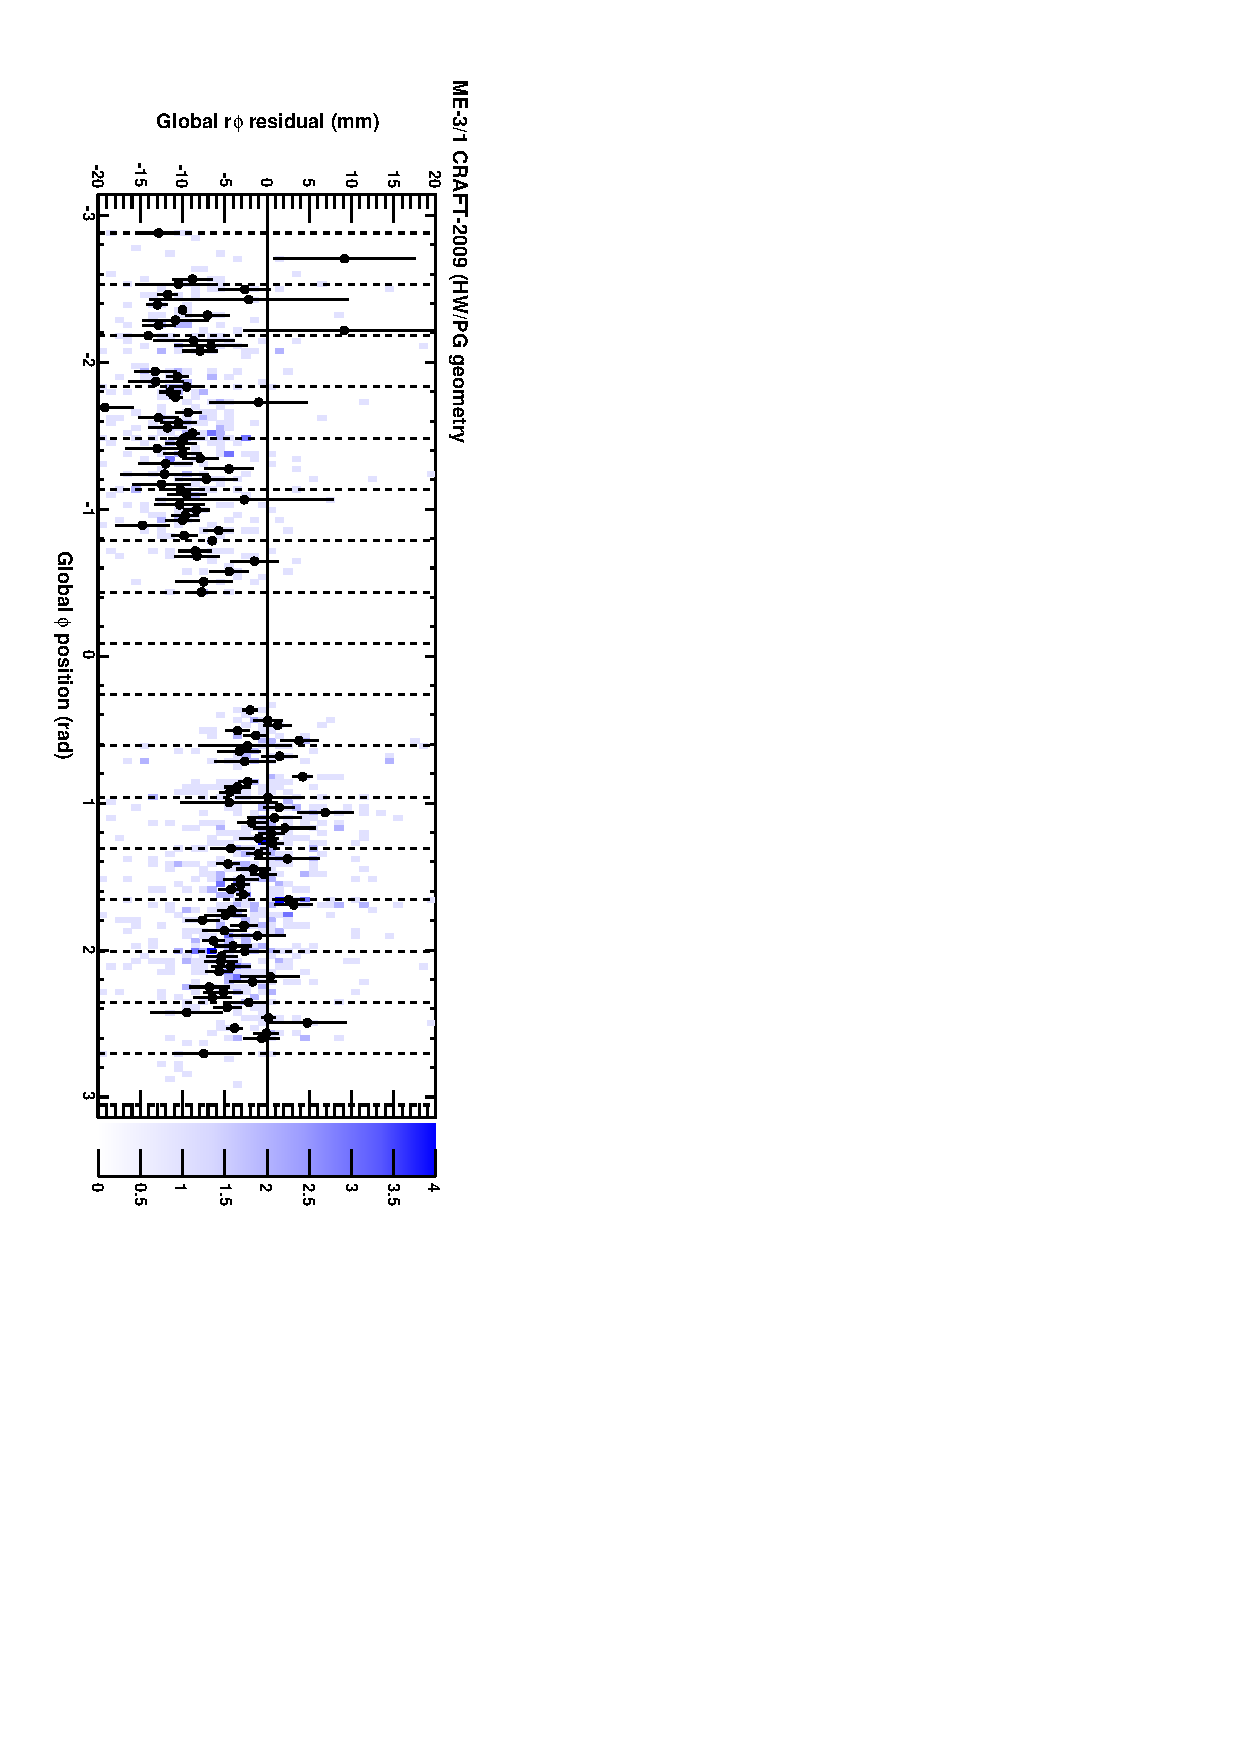
\includegraphics[height=\linewidth, angle=90]{series02.pdf}
\end{frame}

\begin{frame}
\vspace{1 cm}
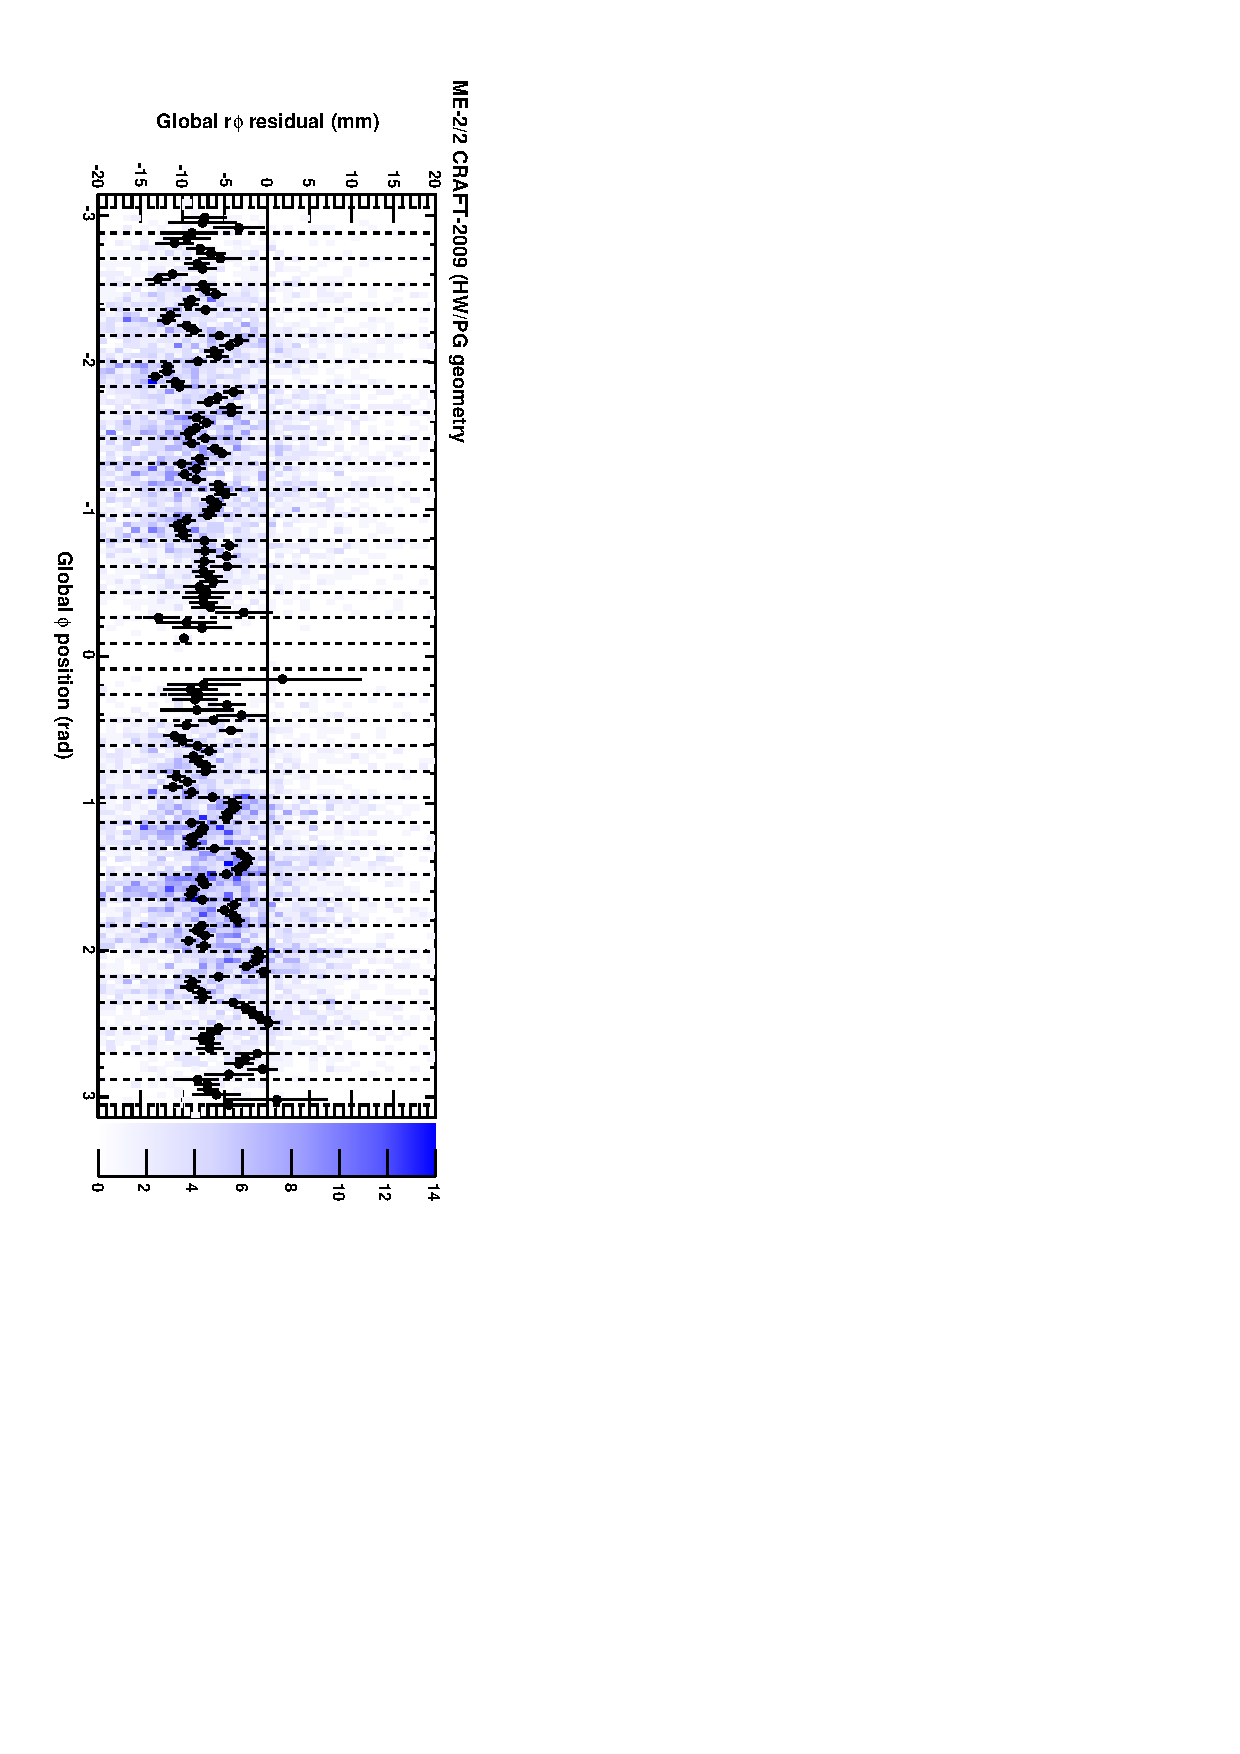
\includegraphics[height=\linewidth, angle=90]{series03.pdf}

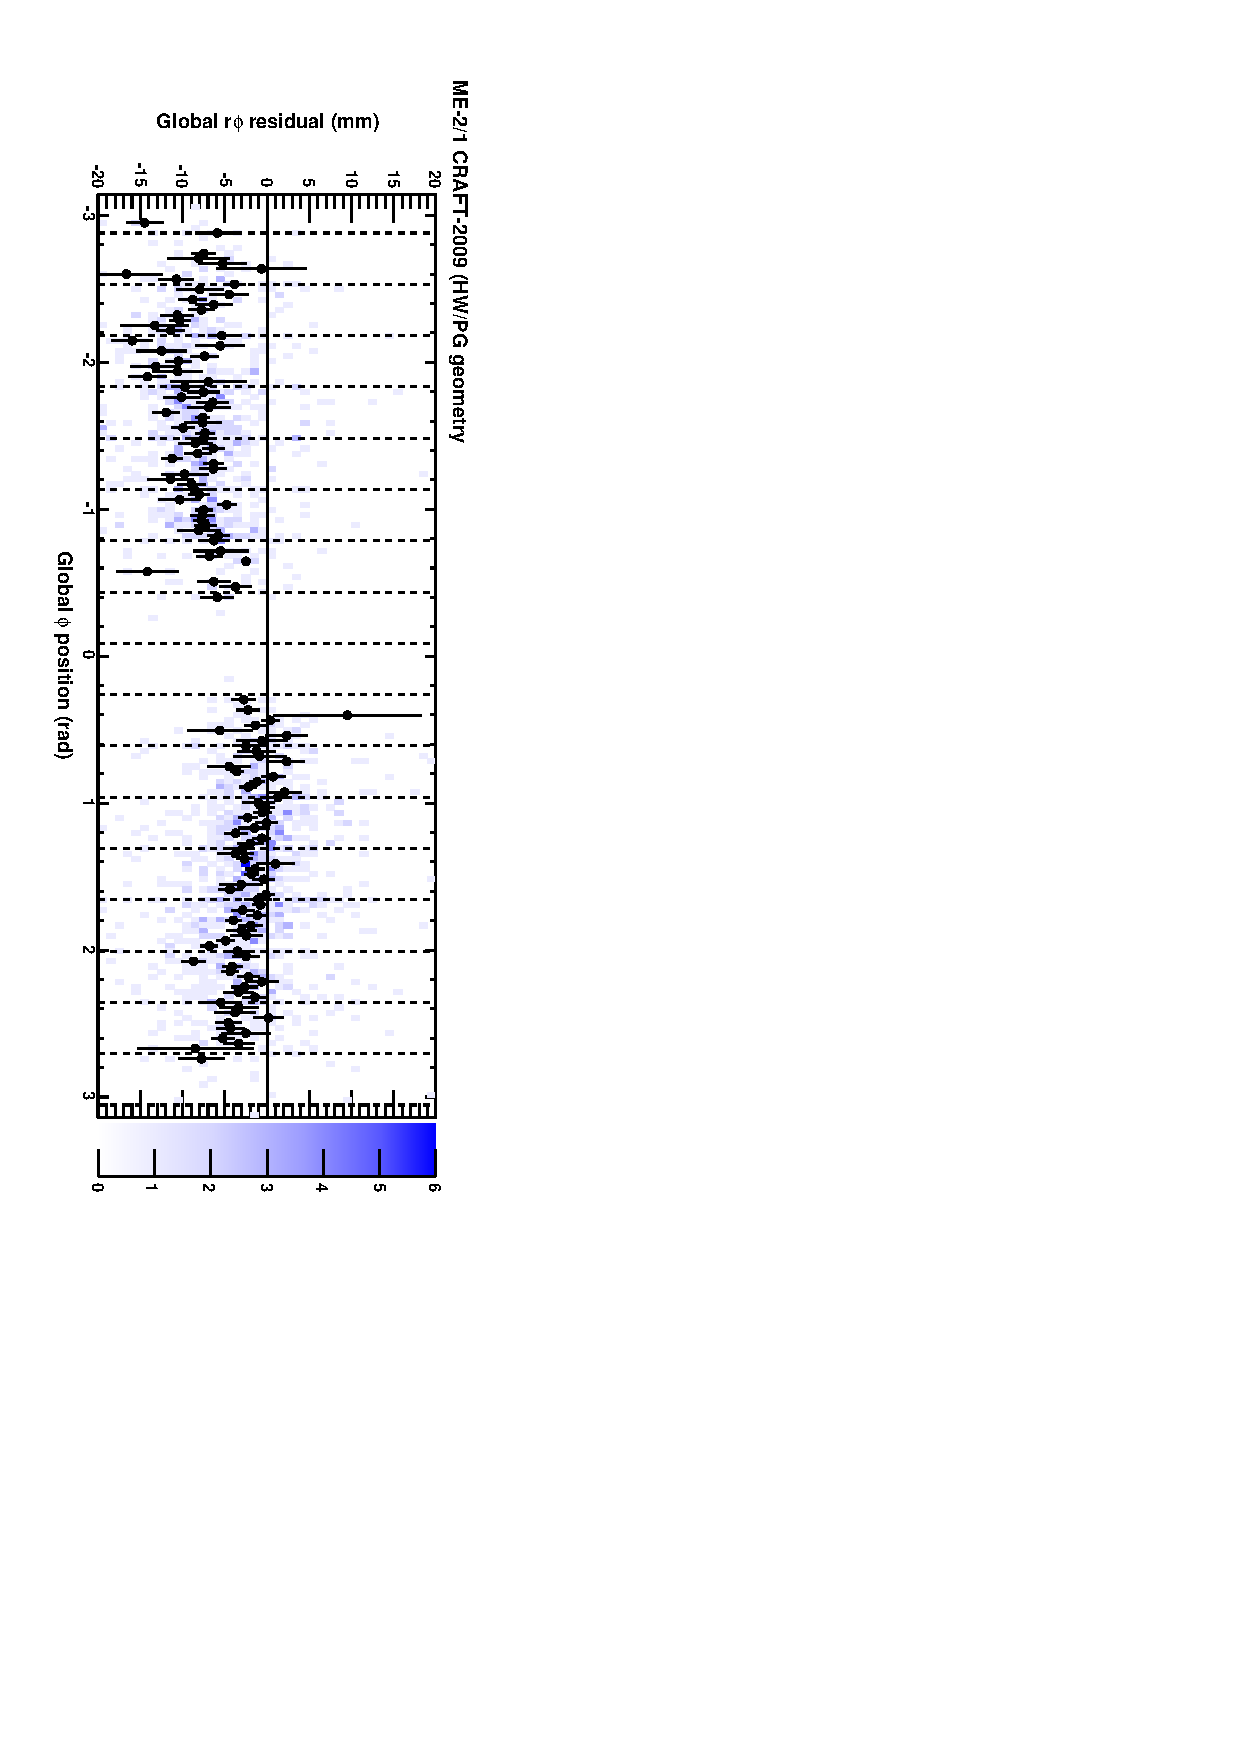
\includegraphics[height=\linewidth, angle=90]{series04.pdf}
\end{frame}

\begin{frame}
\vspace{0.5\baselineskip}
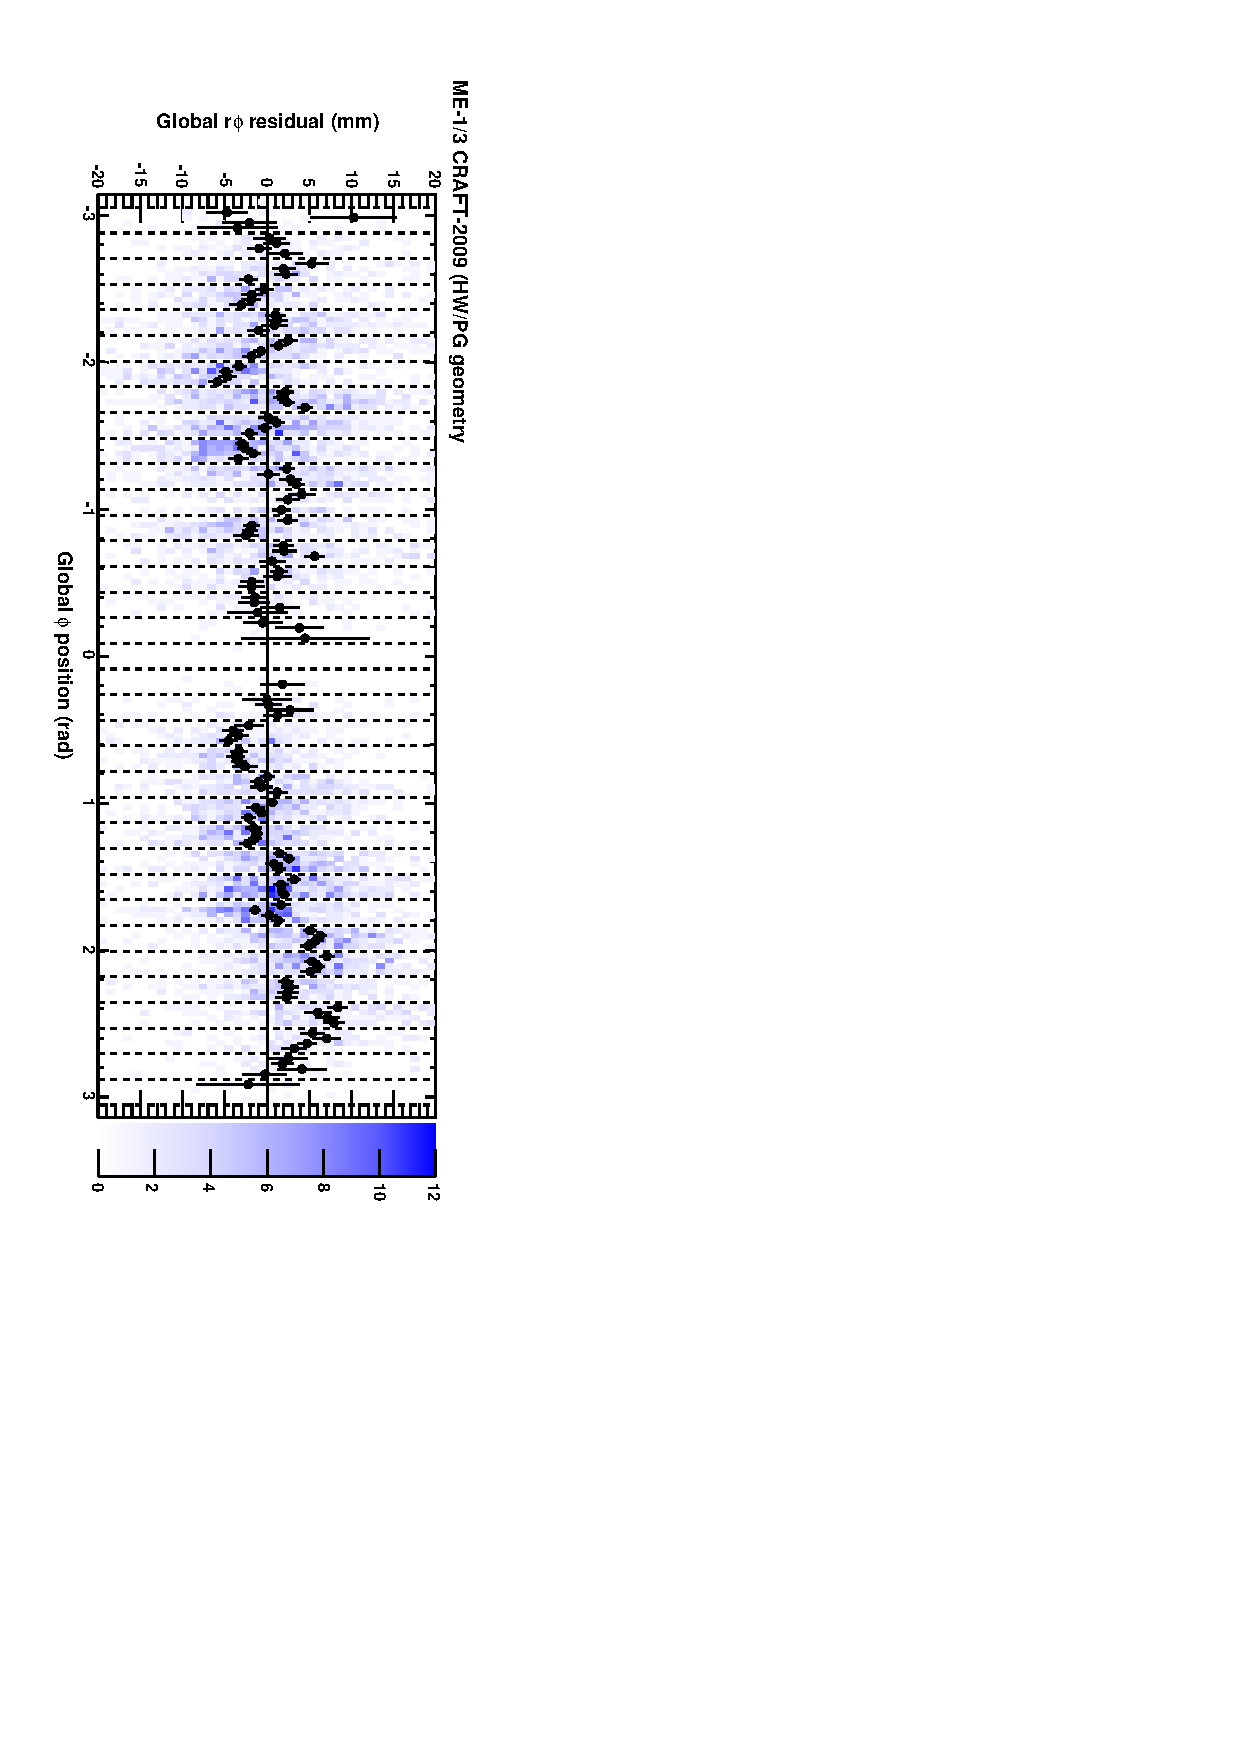
\includegraphics[height=0.75\linewidth, angle=90]{series05.pdf}

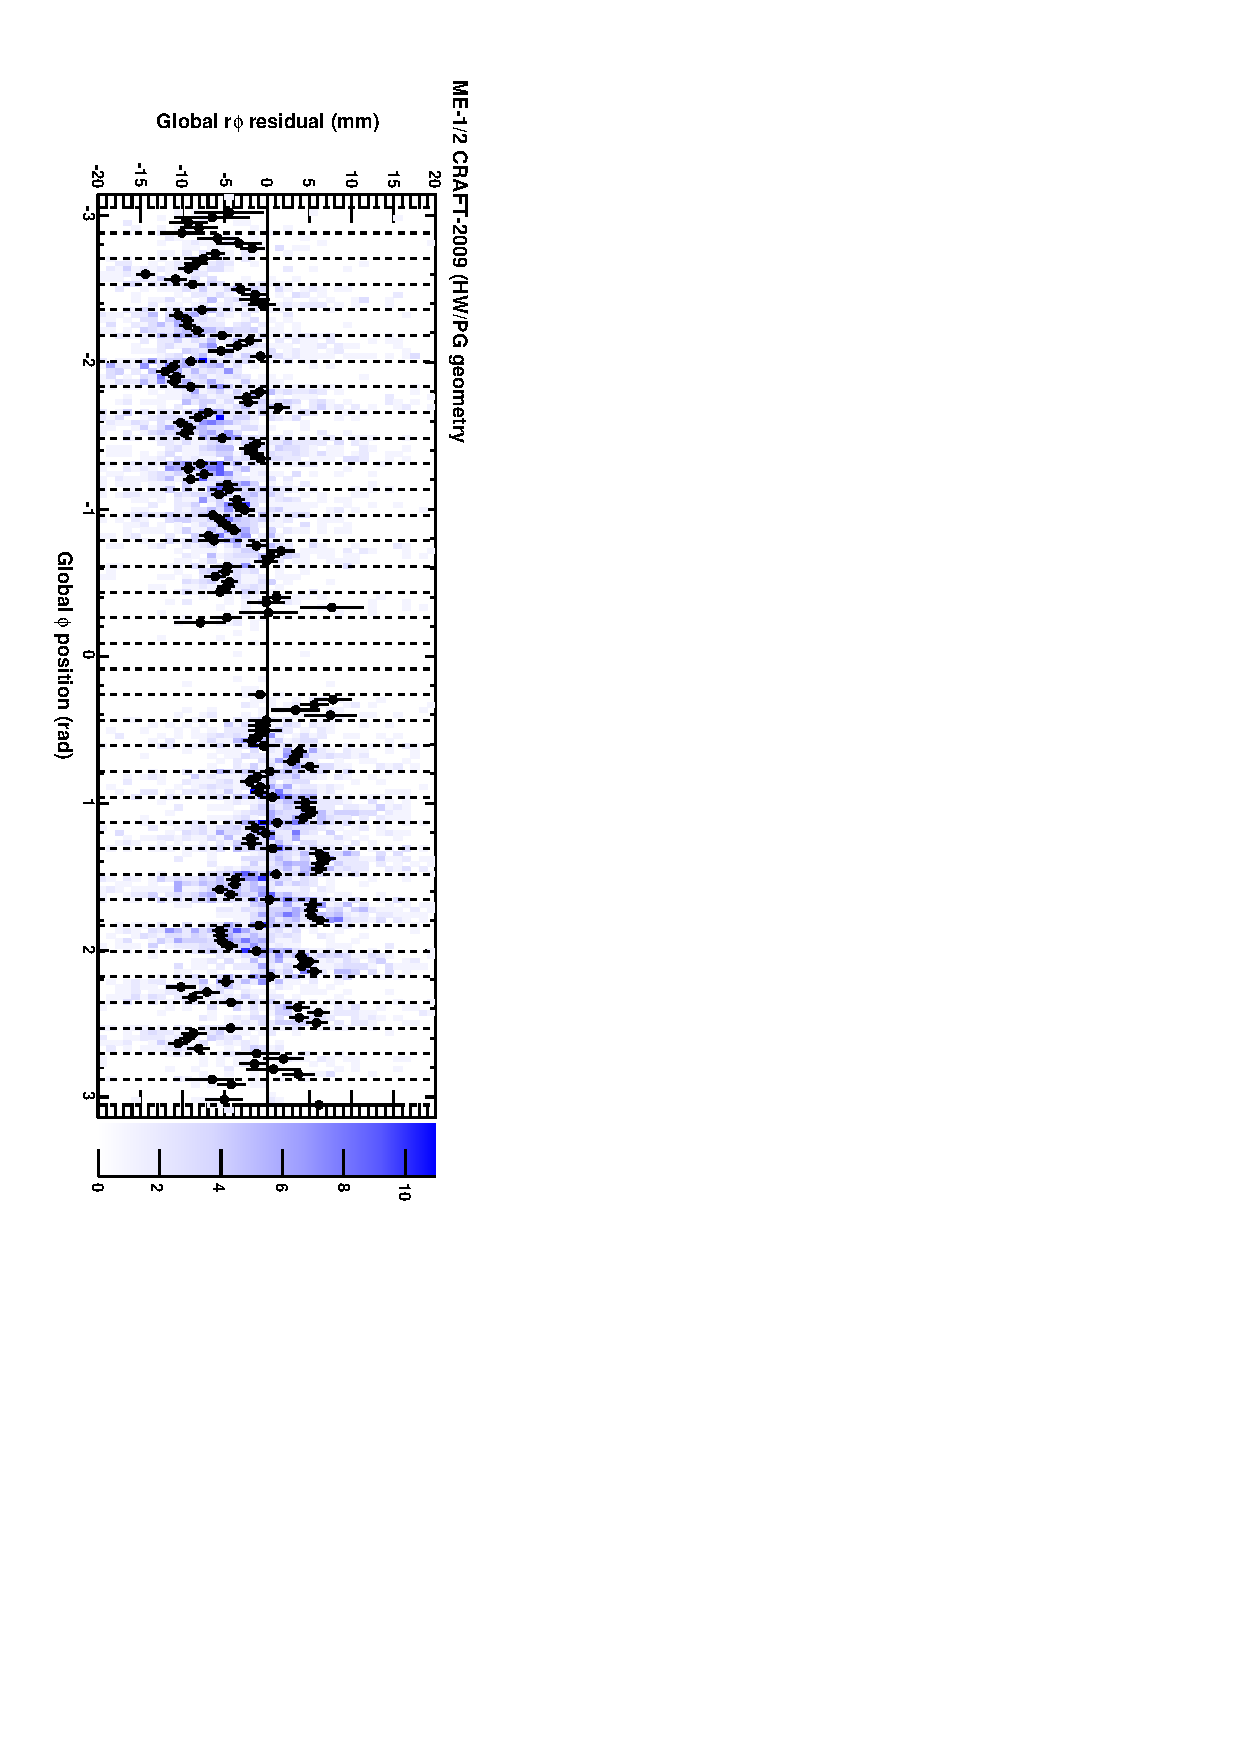
\includegraphics[height=0.75\linewidth, angle=90]{series06.pdf}

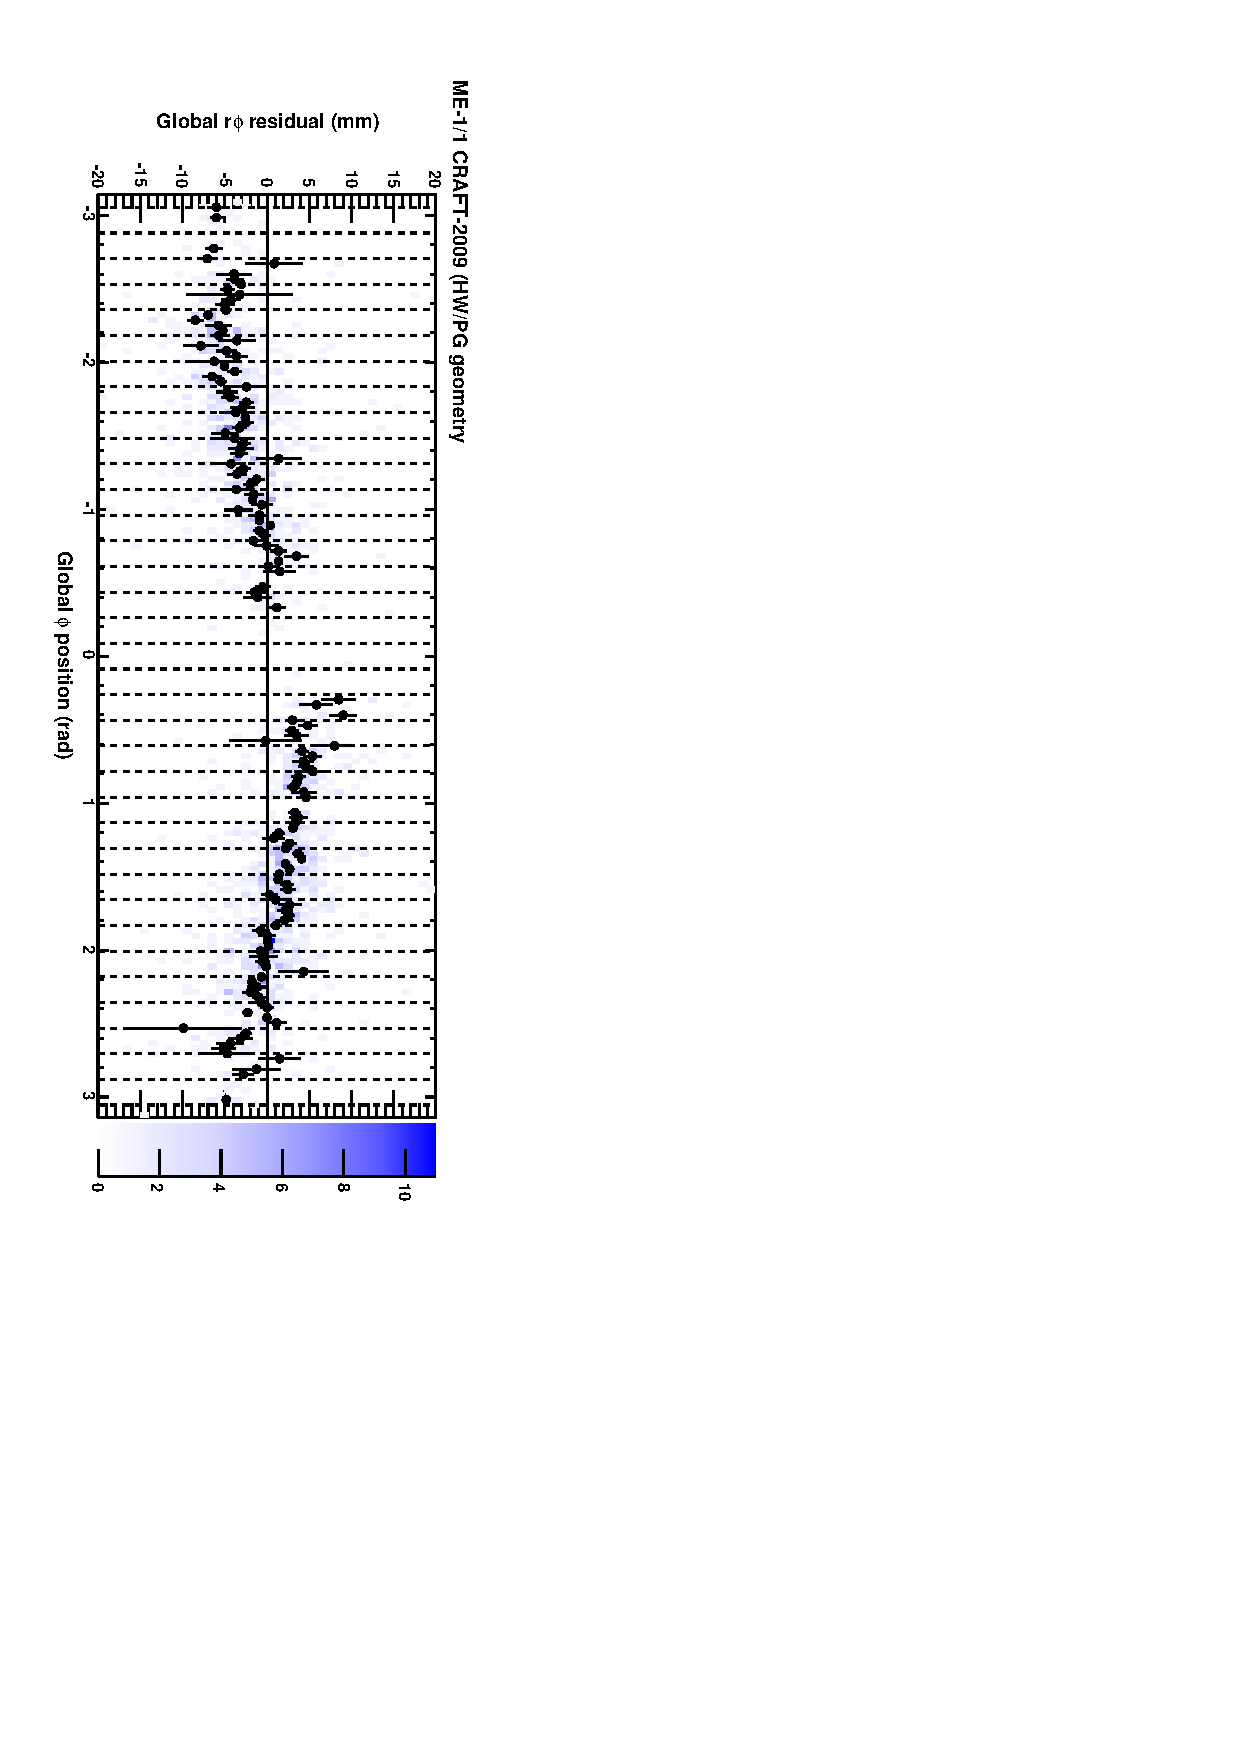
\includegraphics[height=0.75\linewidth, angle=90]{series07.pdf}
\end{frame}

\begin{frame}
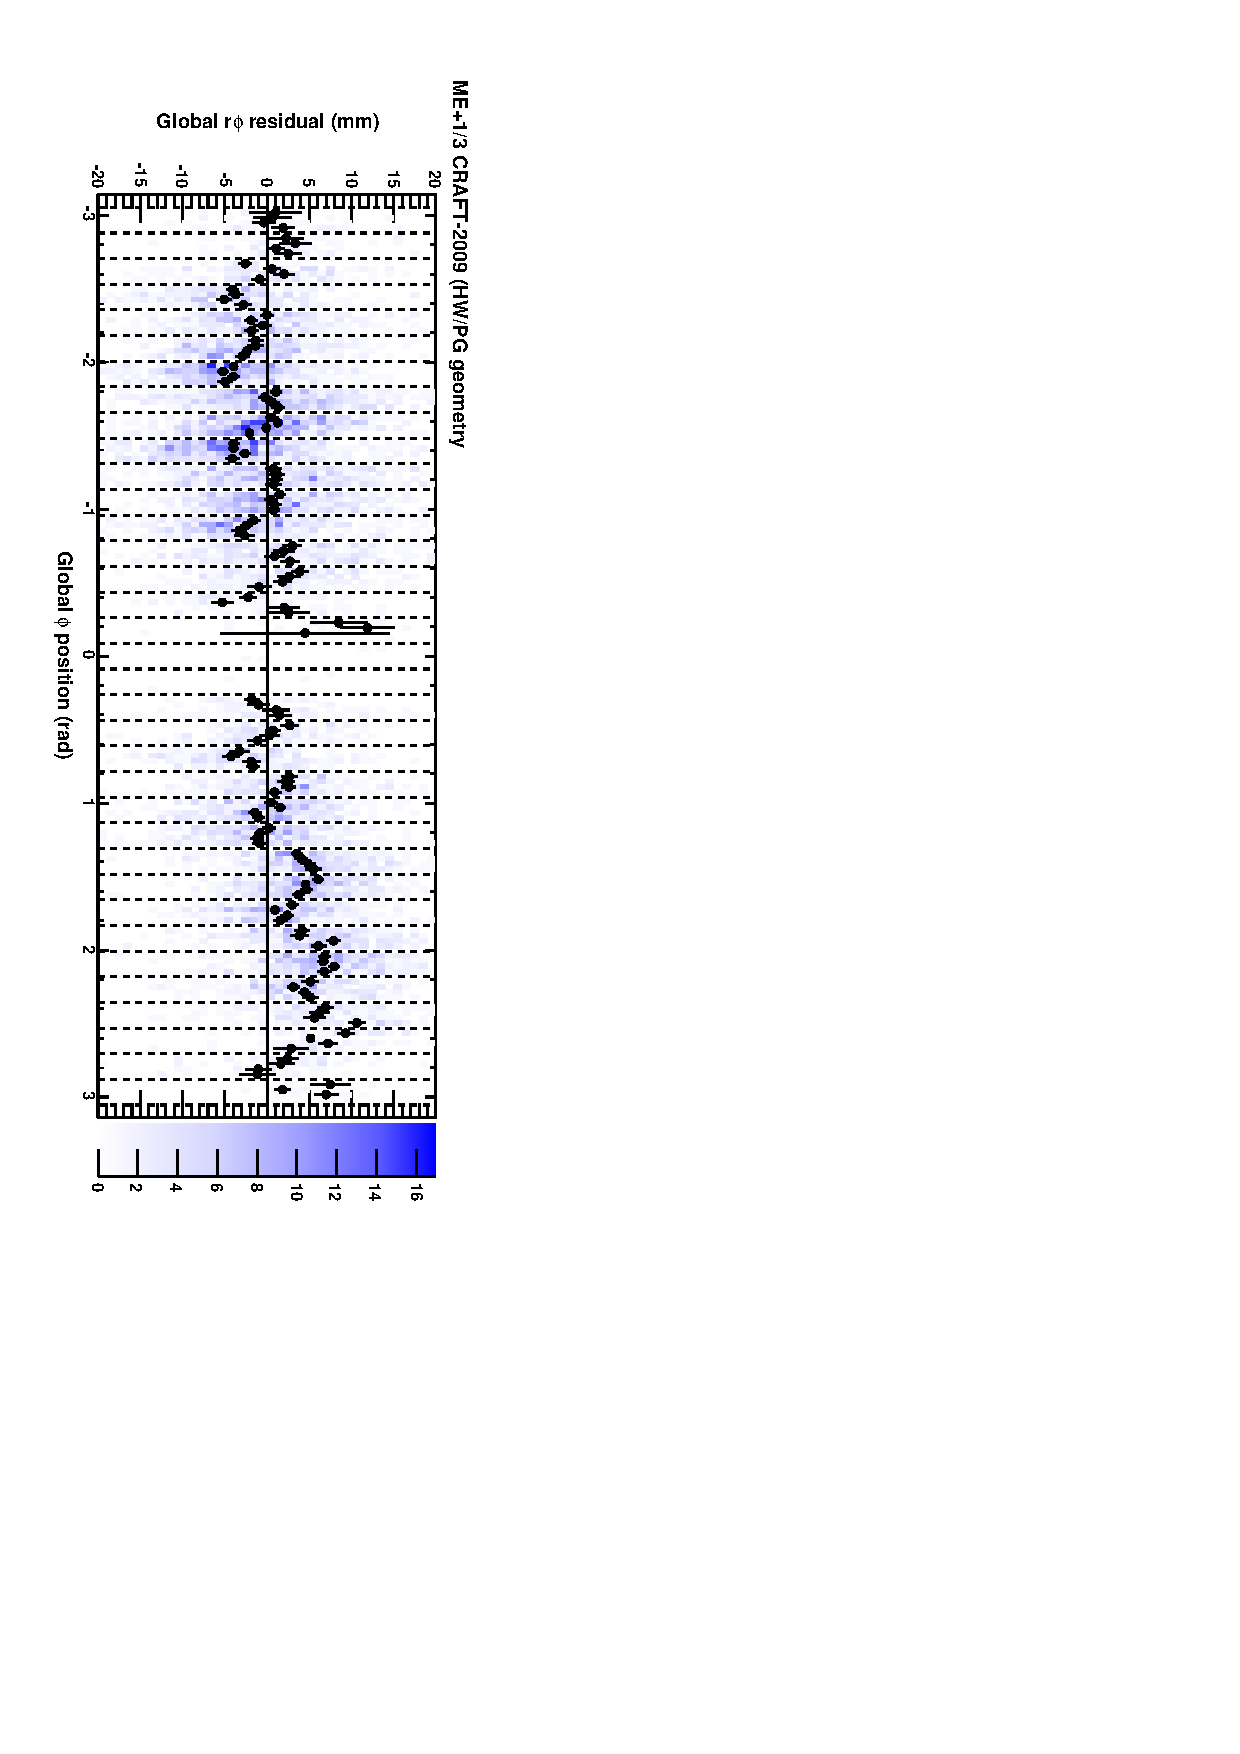
\includegraphics[height=0.75\linewidth, angle=90]{series10.pdf}

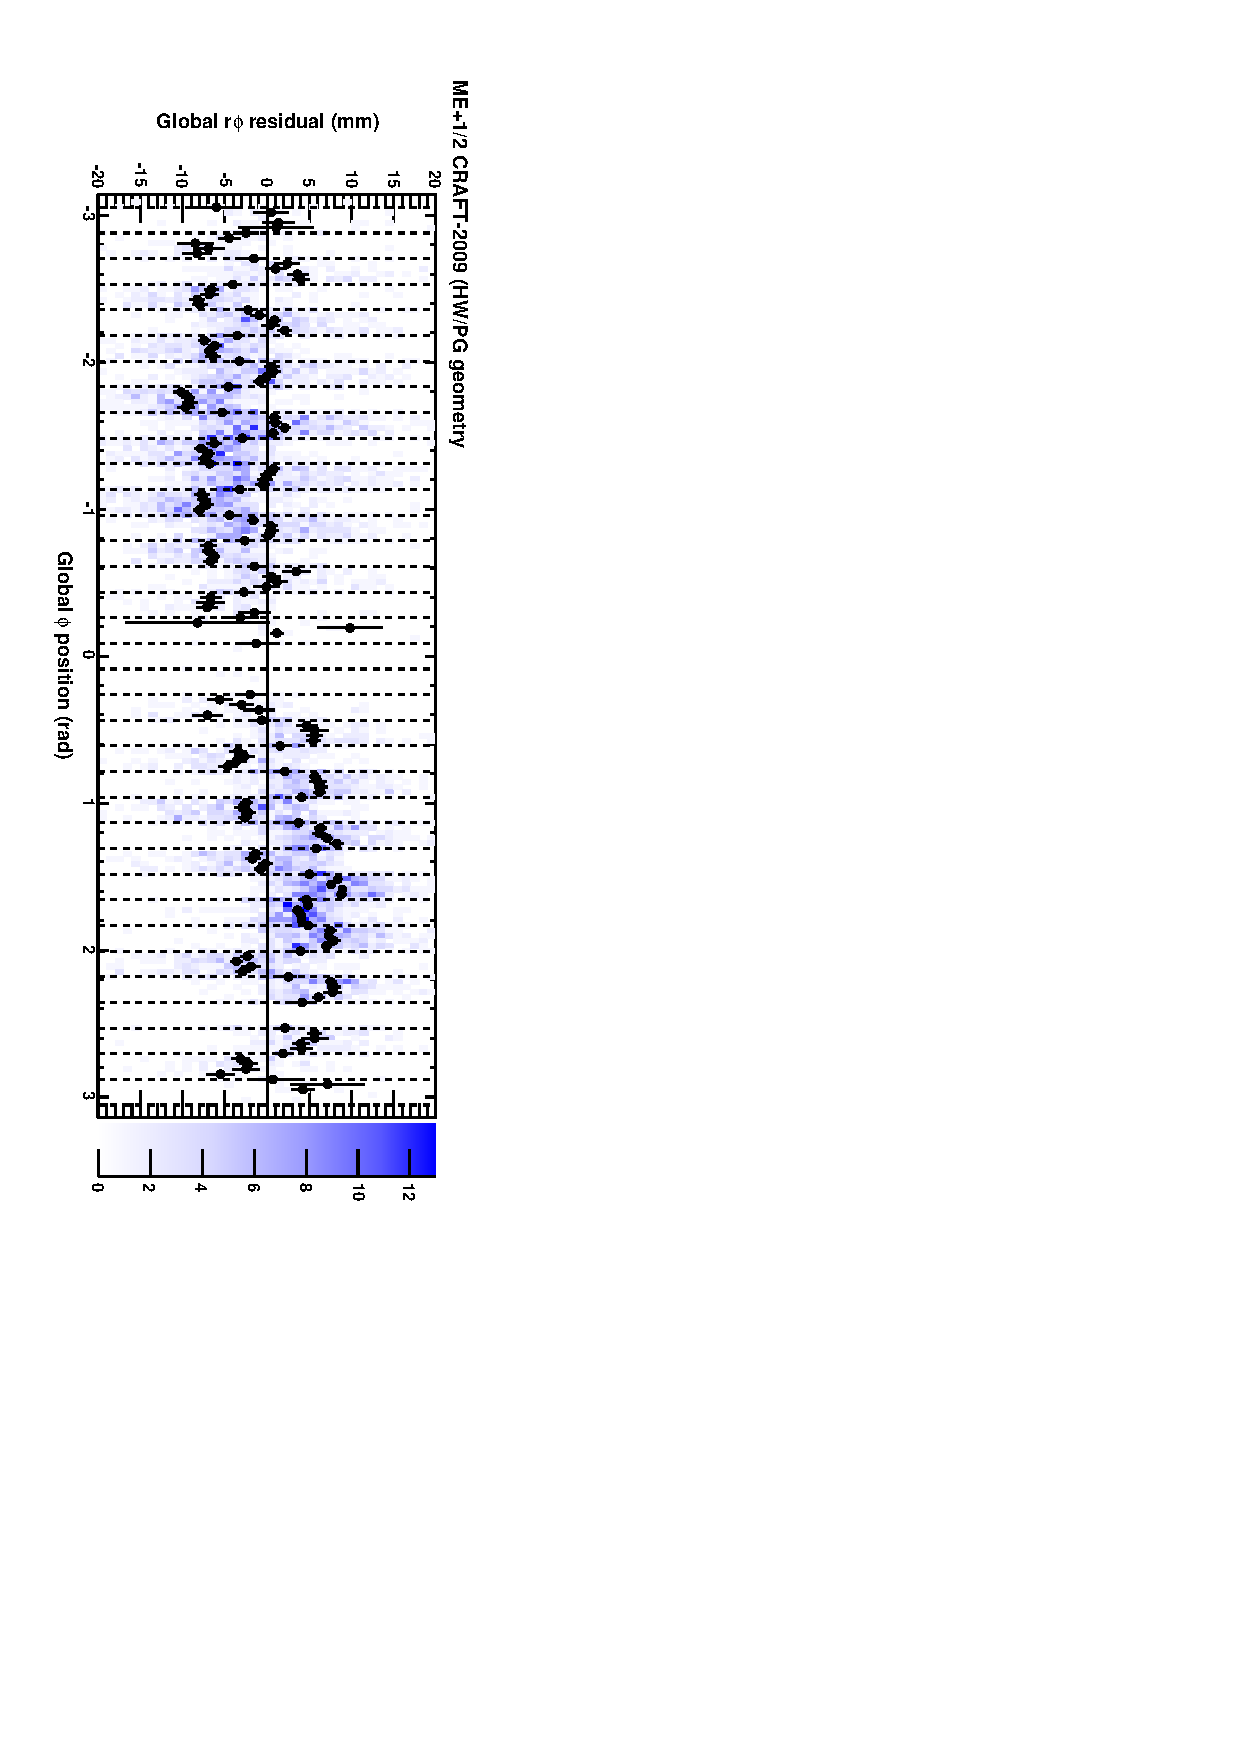
\includegraphics[height=0.75\linewidth, angle=90]{series09.pdf}

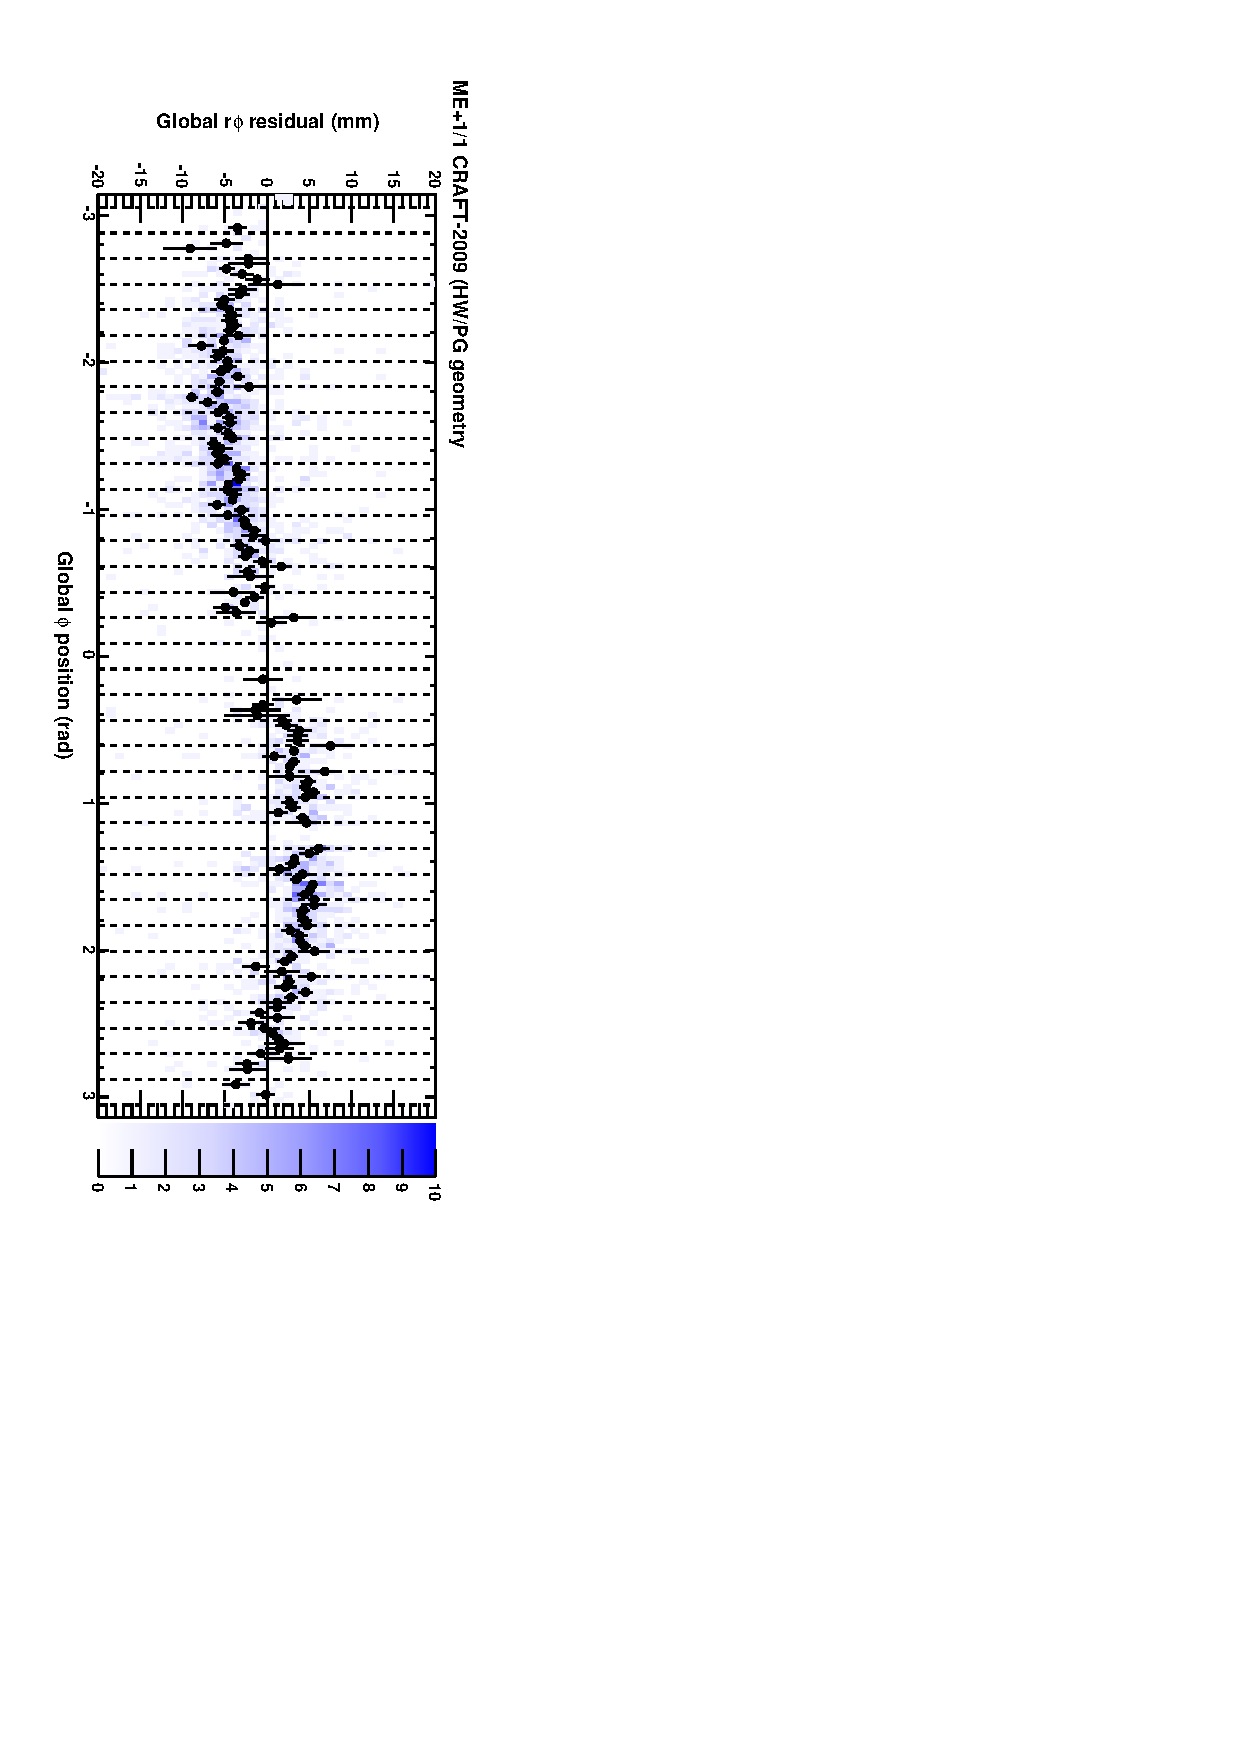
\includegraphics[height=0.75\linewidth, angle=90]{series08.pdf}

\vspace{-2.2 cm}
\hfill clear 5~mm

\hfill $x$ translation

\vspace{2.2 cm}
\vspace{-\baselineskip}
\vspace{-\baselineskip}
\vspace{-\baselineskip}
\vspace{-\baselineskip}
\mbox{ }
\end{frame}

\begin{frame}
\vspace{1 cm}
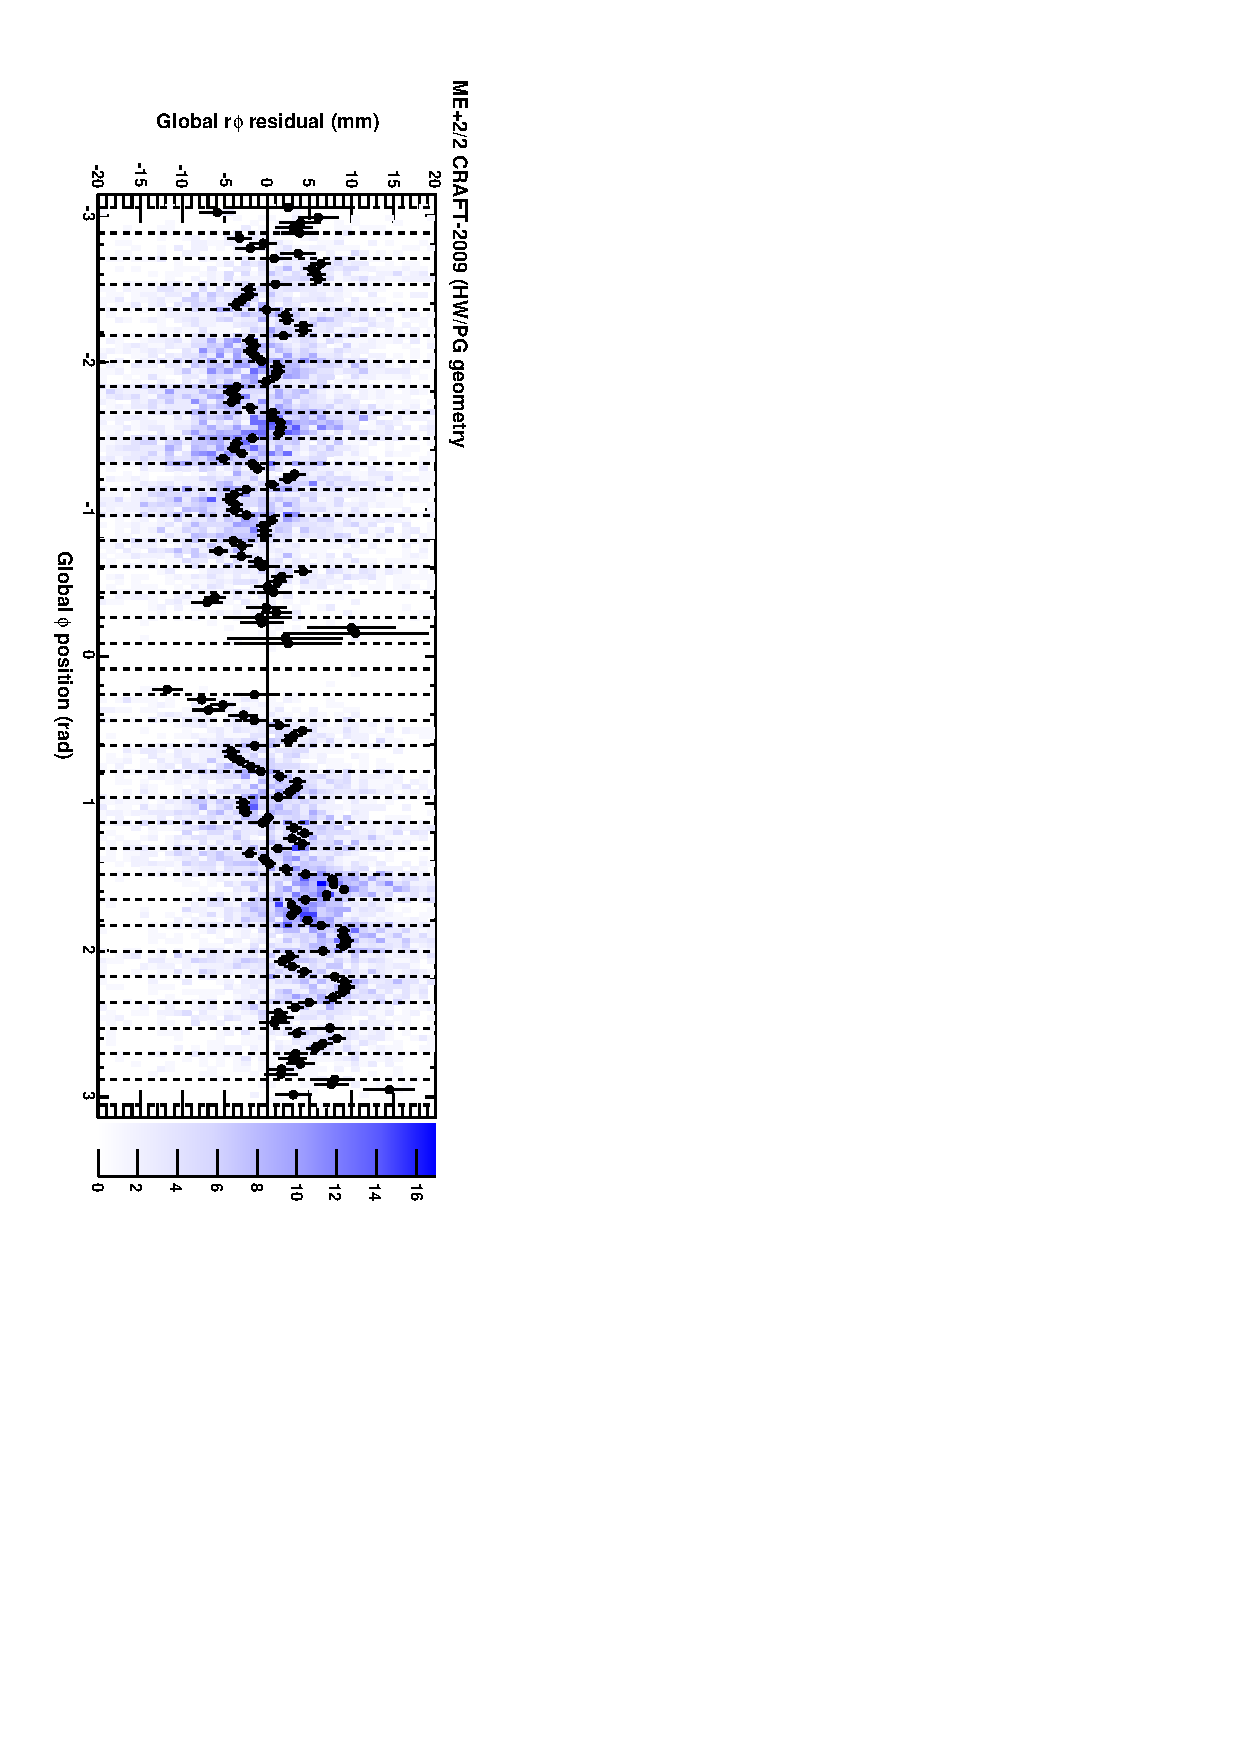
\includegraphics[height=\linewidth, angle=90]{series12.pdf}

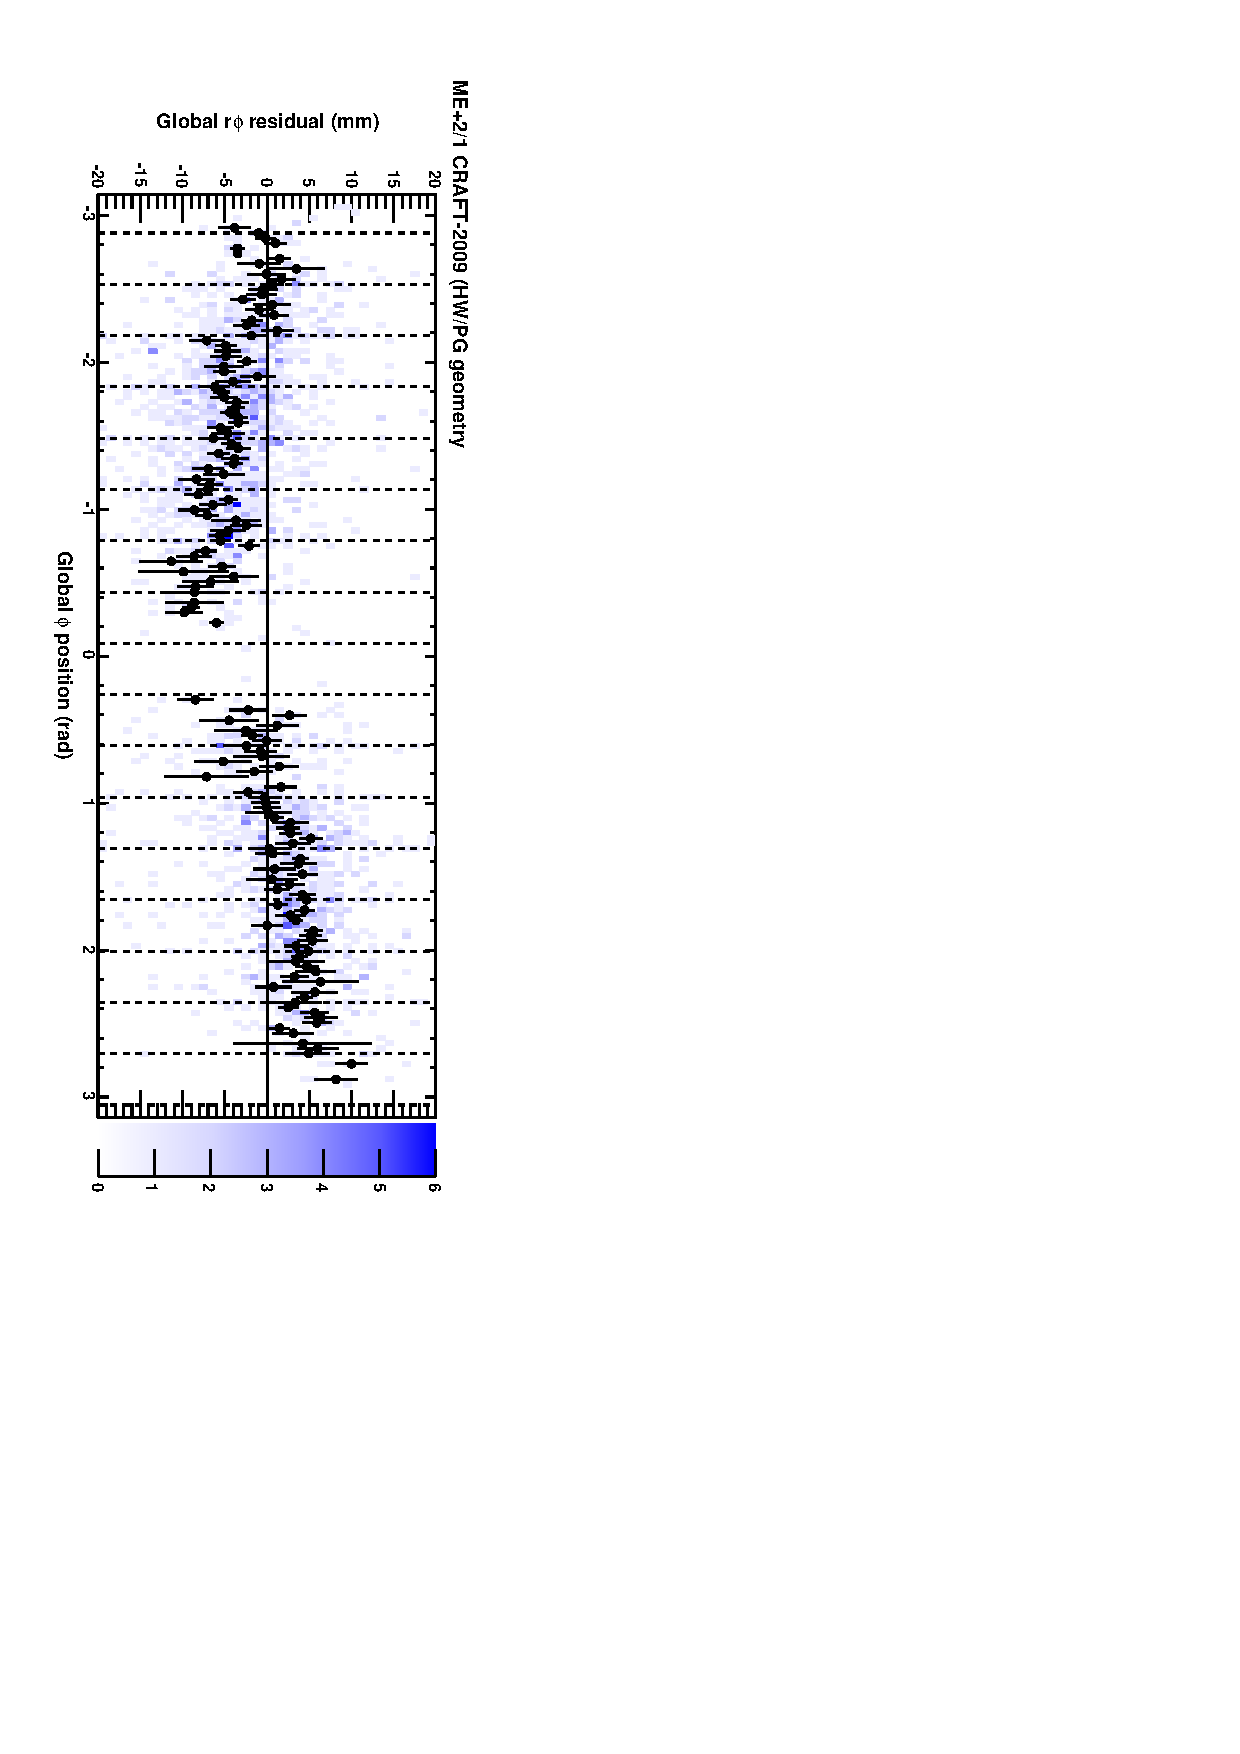
\includegraphics[height=\linewidth, angle=90]{series11.pdf}
\end{frame}

\begin{frame}
\vspace{1 cm}
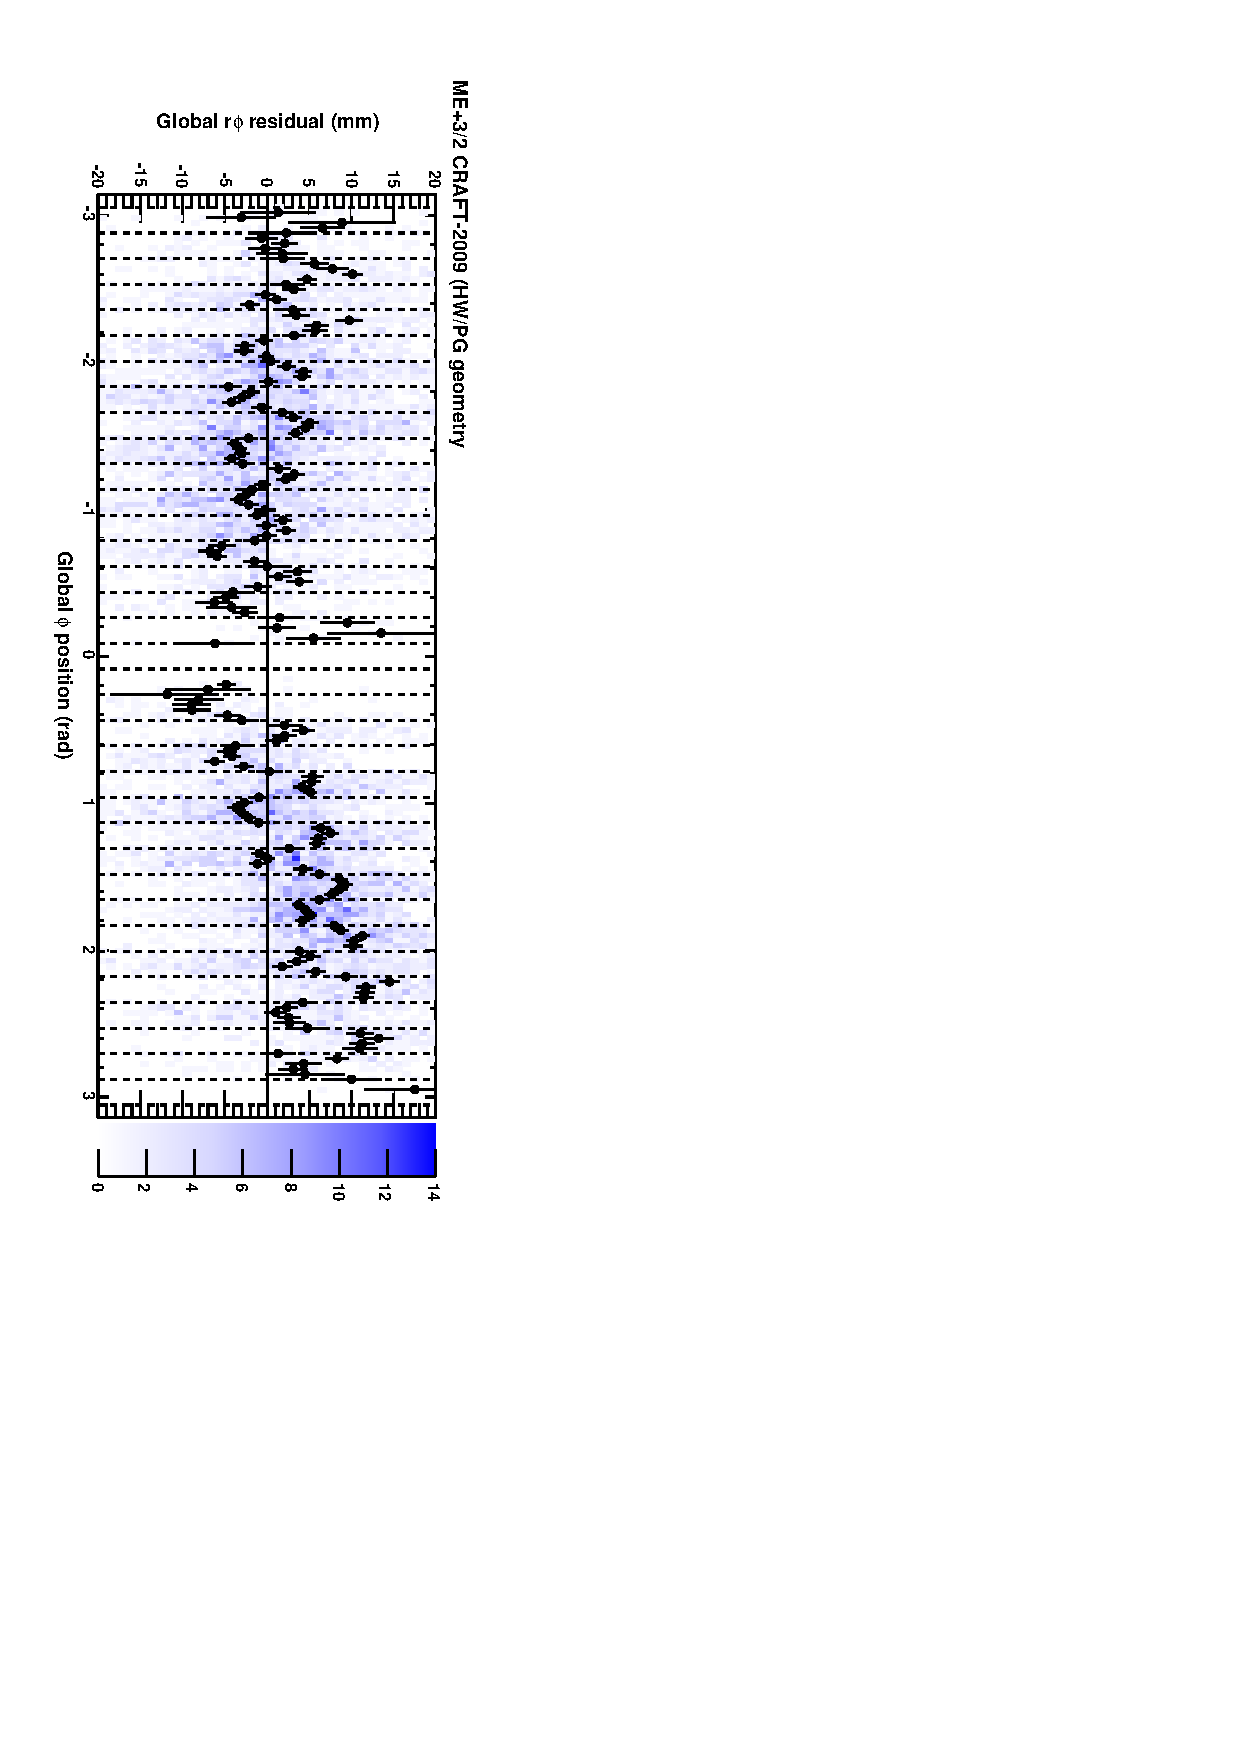
\includegraphics[height=\linewidth, angle=90]{series14.pdf}

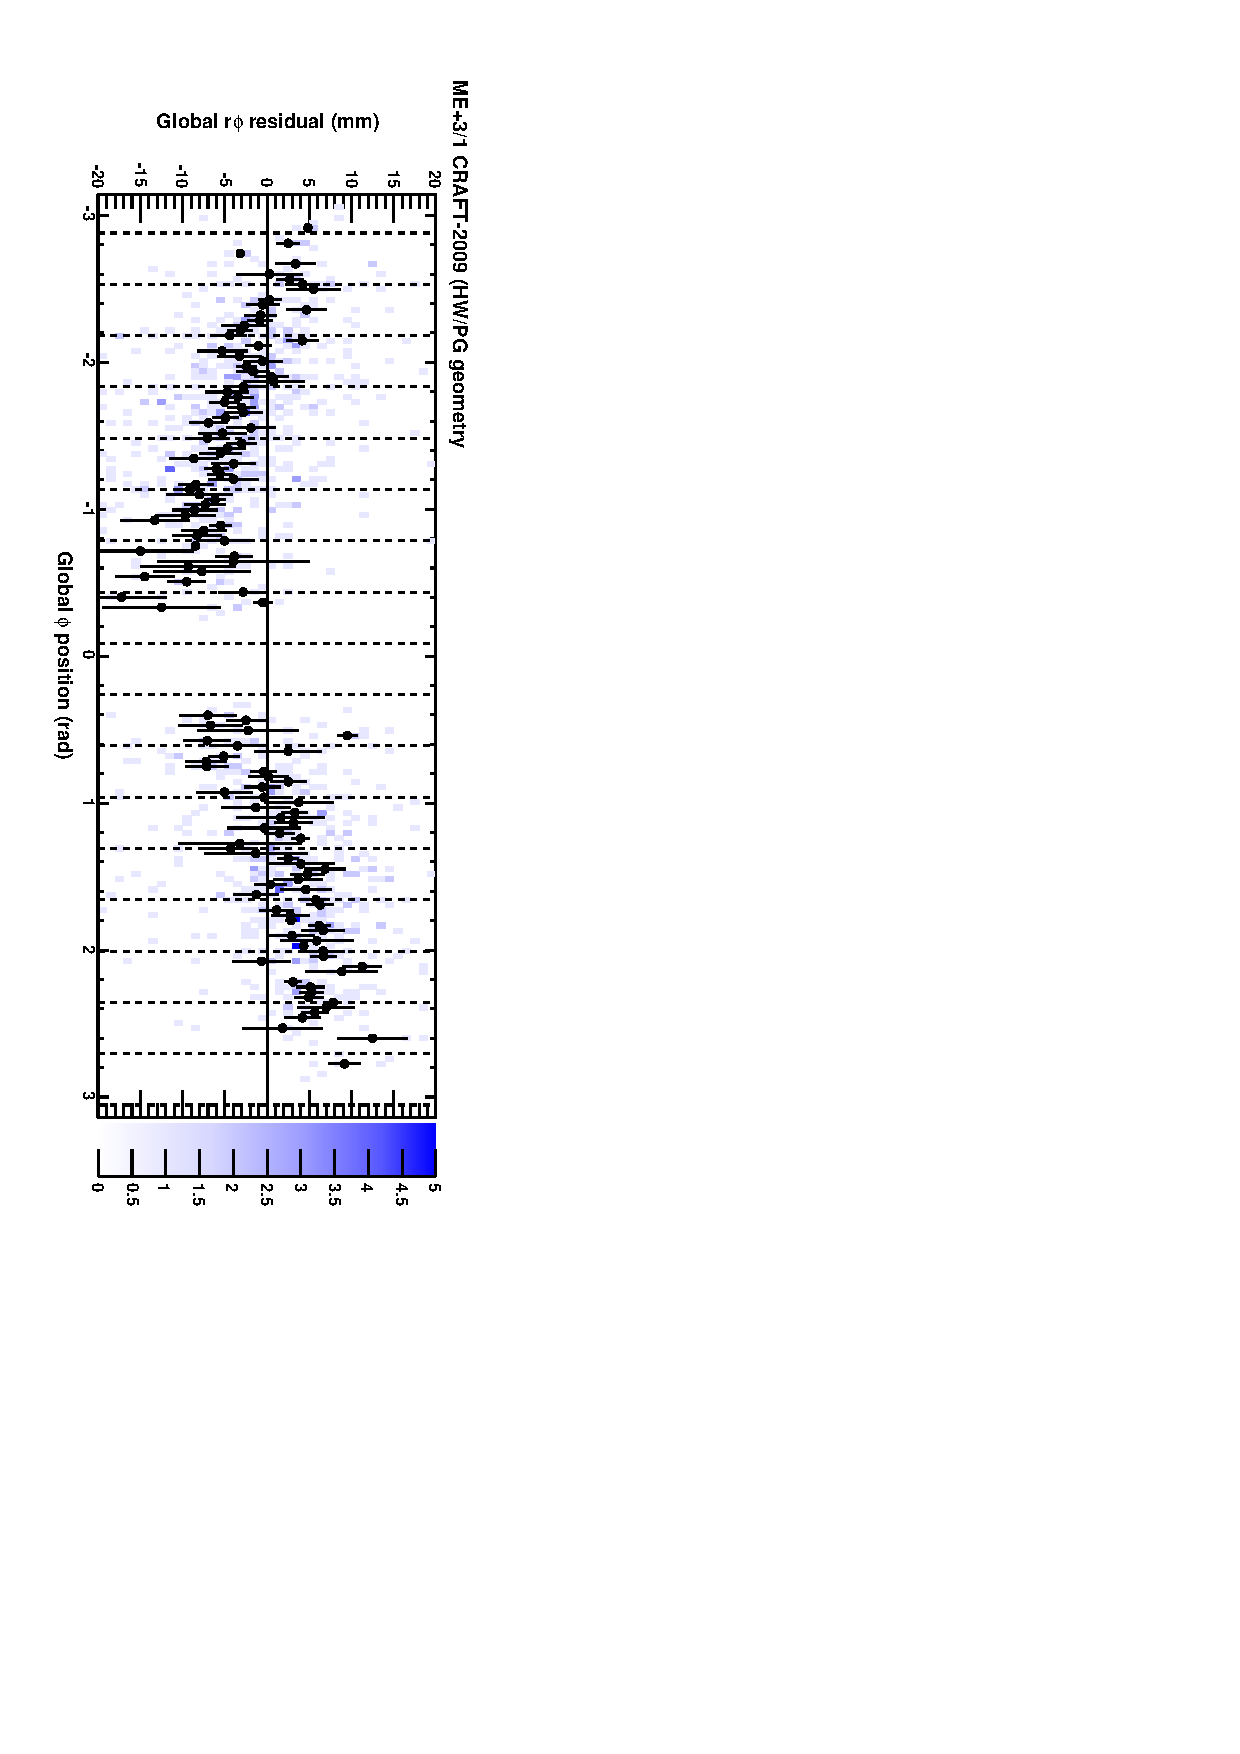
\includegraphics[height=\linewidth, angle=90]{series13.pdf}
\end{frame}

\end{document}
